\graphicspath{{Chapters/CrossSection/Figures/}}
\chapter{Observed Events and \CX\ Measurement}
\chaptermark{\CX\ Measurement}
\label{chap:CrossSection}

\section{Observed Events}

The expected and observed event yields after applying the \ZZ\ and \ZZs\ selections are shown
in~\tab{obs-expected-events-seven} for the 7~\tev\ analysis and
in~\tab{obs-expected-events-eight} for the 8~\tev\ analysis. 
A total
of~\ZZSevenTeVNObsZZLLLL\ events
are observed in \LumiPassGRLTwentyEleven~\ifb\ of 7~\tev\ data for the \ZZ\
selection, and a total of~\ZZSevenTeVNObsZZsLLLL\ events for the \ZZs\ selection. In the 8~\tev\ data, which corresponds to an integrated luminosity of
\LumiPassGRLTwentyTwelve~\ifb, \ZZEightTeVNObsZZLLLL\ events are observed for
the \ZZ\ selection.
%and \ZZEightTeVNObsZZsLLLL\ for the \ZZs\ selection.

%% Expected and observed events, 7 TeV
\begin{table}
\centering
\small
  \begin{tabular}{lcccc}
    \hline\hline
     7~\tev, \ZZ             & \eeee & \mmmm & \eemm & \llll \\
     \hline
Observed & 16 & 23 & 27 & 66 \\
% Systematic is reco+gen_diff+pdf+scale
Exp. Signal &   
    \ZZSevenTeVNExpZZEEEEOneDp~\errSym{\ZZSevenTeVNExpStatZZEEEEOneDp}~\errSym{\ZZSevenTeVNExpSystZZEEEEOneDp} & 
    \ZZSevenTeVNExpZZMMMMOneDp~\errSym{\ZZSevenTeVNExpStatZZMMMMOneDp}~\errSym{\ZZSevenTeVNExpSystZZMMMMOneDp} & 
    \ZZSevenTeVNExpZZEEMMOneDp~\errSym{\ZZSevenTeVNExpStatZZEEMMOneDp}~\errSym{\ZZSevenTeVNExpSystZZEEMMOneDp} & 
    \ZZSevenTeVNExpZZLLLLOneDp~\errSym{\ZZSevenTeVNExpStatZZLLLLOneDp}~\errSym{\ZZSevenTeVNExpSystZZLLLLOneDp} \\
Exp. Bg. & 
    \ZZSevenTeVTotalBgEstZZEEEE &
    \ZZSevenTeVTotalBgEstZZMMMM &
    \ZZSevenTeVTotalBgEstZZEEMM &
    \ZZSevenTeVTotalBgEstZZLLLL \\
\hline\hline
    \\
    \hline\hline
     7~\tev, \ZZs             & \eeee & \mmmm & \eemm & \llll \\
     \hline
Observed & 21 & 30 & 33 & 84 \\
% Systematic is reco+gen_diff+pdf+scale
Exp. Signal &   
    \ZZSevenTeVNExpZZsEEEEOneDp~\errSym{\ZZSevenTeVNExpStatZZsEEEEOneDp}~\errSym{\ZZSevenTeVNExpSystZZsEEEEOneDp} & 
    \ZZSevenTeVNExpZZsMMMMOneDp~\errSym{\ZZSevenTeVNExpStatZZsMMMMOneDp}~\errSym{\ZZSevenTeVNExpSystZZsMMMMOneDp} & 
    \ZZSevenTeVNExpZZsEEMMOneDp~\errSym{\ZZSevenTeVNExpStatZZsEEMMOneDp}~\errSym{\ZZSevenTeVNExpSystZZsEEMMOneDp} & 
    \ZZSevenTeVNExpZZsLLLLOneDp~\errSym{\ZZSevenTeVNExpStatZZsLLLLOneDp}~\errSym{\ZZSevenTeVNExpSystZZsLLLLOneDp} \\
Exp. Bg. & 
    \ZZSevenTeVTotalBgEstZZsEEEE &
    \ZZSevenTeVTotalBgEstZZsMMMM &
    \ZZSevenTeVTotalBgEstZZsEEMM &
    \ZZSevenTeVTotalBgEstZZsLLLL \\
    \hline\hline
  \end{tabular}

      \caption[Expected and observed events in \LumiPassGRLTwentyEleven~\ifb\ of
      7~\tev\ data.]
      {Number of observed events passing the \ZZ\ (top table) and \ZZs\
      (bottom table) selections in \LumiPassGRLTwentyEleven~\ifb\ of 7~\tev\
      data, as well as the expected number of signal events (Exp.~Signal) and
      the expected background (Exp.~Bg.).  The expected background is the sum of
      the data driven estimate for the reducible background and the \mc\
      estimate for the irreducible background. The first uncertainty is statistical, while the second is
      systematic; uncertainties on the integrated luminosity
      (\LumiUncTwentyEleven) are not included.  }
\label{table:obs-expected-events-seven}
\end{table}

%% Expected and observed events, 8 TeV
\begin{table}
\centering
\small
  \begin{tabular}{lcccc}
    \hline\hline
     8~\tev, \ZZ             & \eeee & \mmmm & \eemm & \llll \\
     \hline
Observed & \ZZEightTeVNObsZZEEEE & \ZZEightTeVNObsZZMMMM & \ZZEightTeVNObsZZEEMM & \ZZEightTeVNObsZZLLLL \\
Exp. Signal &   
    \ZZEightTeVNExpZZEEEEOneDp~\errSym{\ZZEightTeVNExpStatZZEEEEOneDp}~\errSym{\ZZEightTeVNExpSystZZEEEEOneDp} & 
    \ZZEightTeVNExpZZMMMMOneDp~\errSym{\ZZEightTeVNExpStatZZMMMMOneDp}~\errSym{\ZZEightTeVNExpSystZZMMMMOneDp} & 
    \ZZEightTeVNExpZZEEMMOneDp~\errSym{\ZZEightTeVNExpStatZZEEMMOneDp}~\errSym{\ZZEightTeVNExpSystZZEEMMOneDp} & 
    \ZZEightTeVNExpZZLLLLOneDp~\errSym{\ZZEightTeVNExpStatZZLLLLOneDp}~\errSym{\ZZEightTeVNExpSystZZLLLLOneDp} \\
Exp. Bg. & 
    \ZZEightTeVTotalBgEstZZEEEE &
    \ZZEightTeVTotalBgEstZZMMMM &
    \ZZEightTeVTotalBgEstZZEEMM &
    \ZZEightTeVTotalBgEstZZLLLL \\
\hline\hline
%    \\
%    \hline\hline
%     8~\tev, \ZZs             & \eeee & \mmmm & \eemm & \llll \\
%     \hline
%Observed & \ZZEightTeVNObsZZEEEE & \ZZEightTeVNObsZZMMMM & \ZZEightTeVNObsZZEEMM & \ZZEightTeVNObsZZLLLL \\
%Exp. Signal &   
%    \ZZEightTeVNExpZZsEEEE~\errSym{\ZZEightTeVNExpStatZZsEEEE}~\errSym{\ZZEightTeVNExpStatZZsEEEE} & 
%    \ZZEightTeVNExpZZsMMMM~\errSym{\ZZEightTeVNExpStatZZsMMMM}~\errSym{\ZZEightTeVNExpStatZZsMMMM} & 
%    \ZZEightTeVNExpZZsEEMM~\errSym{\ZZEightTeVNExpStatZZsEEMM}~\errSym{\ZZEightTeVNExpStatZZsEEMM} & 
%    \ZZEightTeVNExpZZsLLLL~\errSym{\ZZEightTeVNExpStatZZsLLLL}~\errSym{\ZZEightTeVNExpStatZZsLLLL} \\
%Exp. Bg. & 
%    \ZZEightTeVNBgZZsEEEE~\errSym{\ZZEightTeVNBgStatZZsEEEE}~\errSym{\ZZEightTeVNBgStatZZsEEEE} & 
%    \ZZEightTeVNBgZZsMMMM~\errSym{\ZZEightTeVNBgStatZZsMMMM}~\errSym{\ZZEightTeVNBgStatZZsMMMM} & 
%    \ZZEightTeVNBgZZsEEMM~\errSym{\ZZEightTeVNBgStatZZsEEMM}~\errSym{\ZZEightTeVNBgStatZZsEEMM} & 
%    \ZZEightTeVNBgZZsLLLL~\errSym{\ZZEightTeVNBgStatZZsLLLL}~\errSym{\ZZEightTeVNBgStatZZsLLLL} \\
%    \hline\hline
  \end{tabular}

      \caption[Expected and observed events in \LumiPassGRLTwentyTwelve~\ifb\ of
      8~\tev\ data.]
      {Number of observed events passing the \ZZllll\ (top table) and \ZZsllll\
      (bottom table) selections in \LumiPassGRLTwentyTwelve~\ifb\ of 8~\tev\
      data, as well as the expected number of signal events (Exp.~Signal) and
      the expected background (Exp.~Bg.).  The expected background is the sum of
      the data driven estimate for the reducible background and the \mc\
      estimate for the irreducible background. The first uncertainty is statistical, while the second is
      systematic; uncertainties on the integrated luminosity
      (\LumiUncTwentyTwelve) are not included.  }
    \label{table:obs-expected-events-eight}
\end{table}

\section{Kinematic Distributions}
\label{sec:results-kindists}

\figs{zzdists-Zmass2D-seven}{zzdists-Zmass2D-eight} show the mass of the
subleading \leppair\ versus the mass of the leading \leppair\ for the 7~\tev\
and 8~\tev\ analyses respectively (ordered in \pt; see~\sec{eventsel-definitions}). 
In both cases the solid red box
represents the region defined by the mass requirements of the \ZZ\ selection and
the dashed blue box the region defined by those of the \ZZs\ selection. The
events are seen to cluster in the regions where both masses are near \mZ, in
agreement with the \mc\ prediction for the signal (shown as pink boxes, with the
size of the box proportional to the number of expected events).

\fig{zzdists-dr-ptz-seven} shows the correlation between the transverse momentum
of the \leppair s and the opening-angle between the leptons forming the pair in
the 7~\tev\ data. It is observed that for higher transverse momentum \dilep\
pairs the opening-angle tends to be smaller, in good agreement with the \mc\
predictions. 

\figs{zzdists-Zmass-seven}{zzdists-Zmass-eight} show the \dilep\ invariant mass
distributions for the leading and subleading \leppair\ for the 7~\tev\ and
8~\tev\ analyses. ~\fig{zzdists-ZZ-seven} shows the
transverse momentum $\pT^{\ZZ}$ and invariant mass $m^{\ZZ}$ of the four-lepton
system, the transverse momentum of the leading \dilep\ pair $\pt^{Z1}$, and the
transverse momentum of the subleading \dilep\ pair $\pt^{Z2}$, for events
passing the \ZZ\ selection in the 7~\tev\ data; \fig{zzdists-ZZ-eight}
shows equivalent figure for the 8~\tev\ data.
\fig{zzdists-ZZs-seven} shows the corresponding
distributions for events passing the \ZZs\ selection in the 7~\tev\ data. In
each case, the prediction from \mc\ for
the \ZZ\ signal is shown as a pink histogram and the prediction for the
background
is shown as a light blue histogram. The shapes of the distributions observed in
data are consistent with the predictions.

%~\fig{zzdists-mindr-mzz-seven} shows the minimum 

% 2D plot, 7 TeV
% Use PDF figure as text alignment is off in eps
 \begin{figure}[htbp]
 \begin{center}
  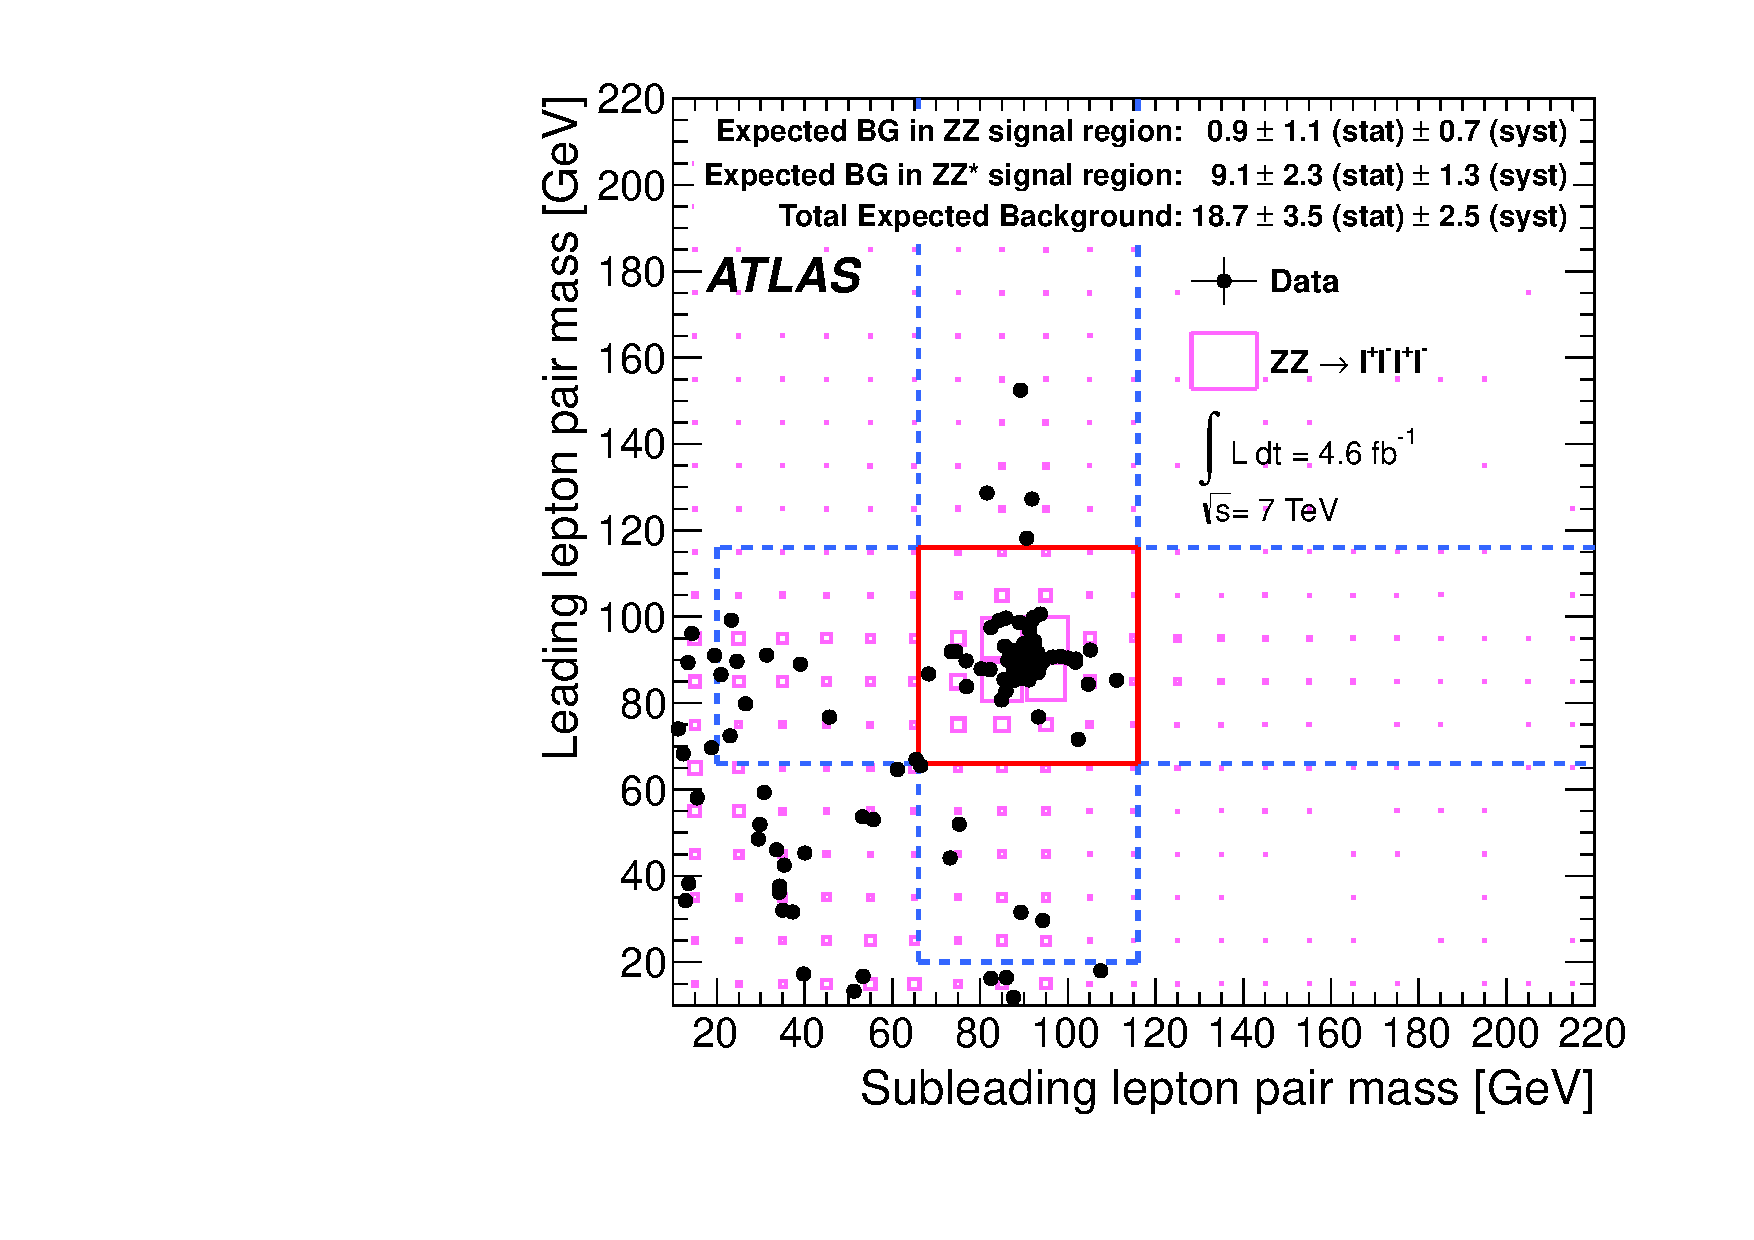
\includegraphics[width=0.9\textwidth]{7TeV/h_mz1_mz2.pdf}\hfill
  \caption[Mass of the leading \leppair\ versus the mass of the
  sub-leading \leppair\ for candidate \ZZ\ events in the 7~\tev\ data.]
  {\small Mass of the leading \leppair\ versus the mass of the
  sub-leading \leppair\ for candidate \ZZ\ events in the 7~\tev\ data after
  applying all of the selection
  requirements apart from the \dilepton\ mass requirements.
  The events observed in the data are shown as solid circles and the \ZZsllll\
  signal prediction from simulation as boxes,
  with the size of each box is proportional to the expected number of events in each bin.  
  The region enclosed by the solid (dashed) lines indicates the signal region defined by the
  \dilepton\ mass requirements for \ZZ\ (\ZZs) events. The expected backgrounds
  quoted in the label are slightly different to those quoted
  in~\tab{bg-est-final} as they refer to the numbers in the published ATLAS
  analysis~\cite{ATLAS:2012kg} which used a different background estimate; the
  expectations are consistent within the uncertainties.
  %The background estimate is described in section 5.1.
   }
    \label{fig:zzdists-Zmass2D-seven}
 \end{center}
 \end{figure}

% 2D plot, 8 TeV
% Use PDF figure as text alignment is off in eps
 \begin{figure}[htbp]
 \begin{center}
  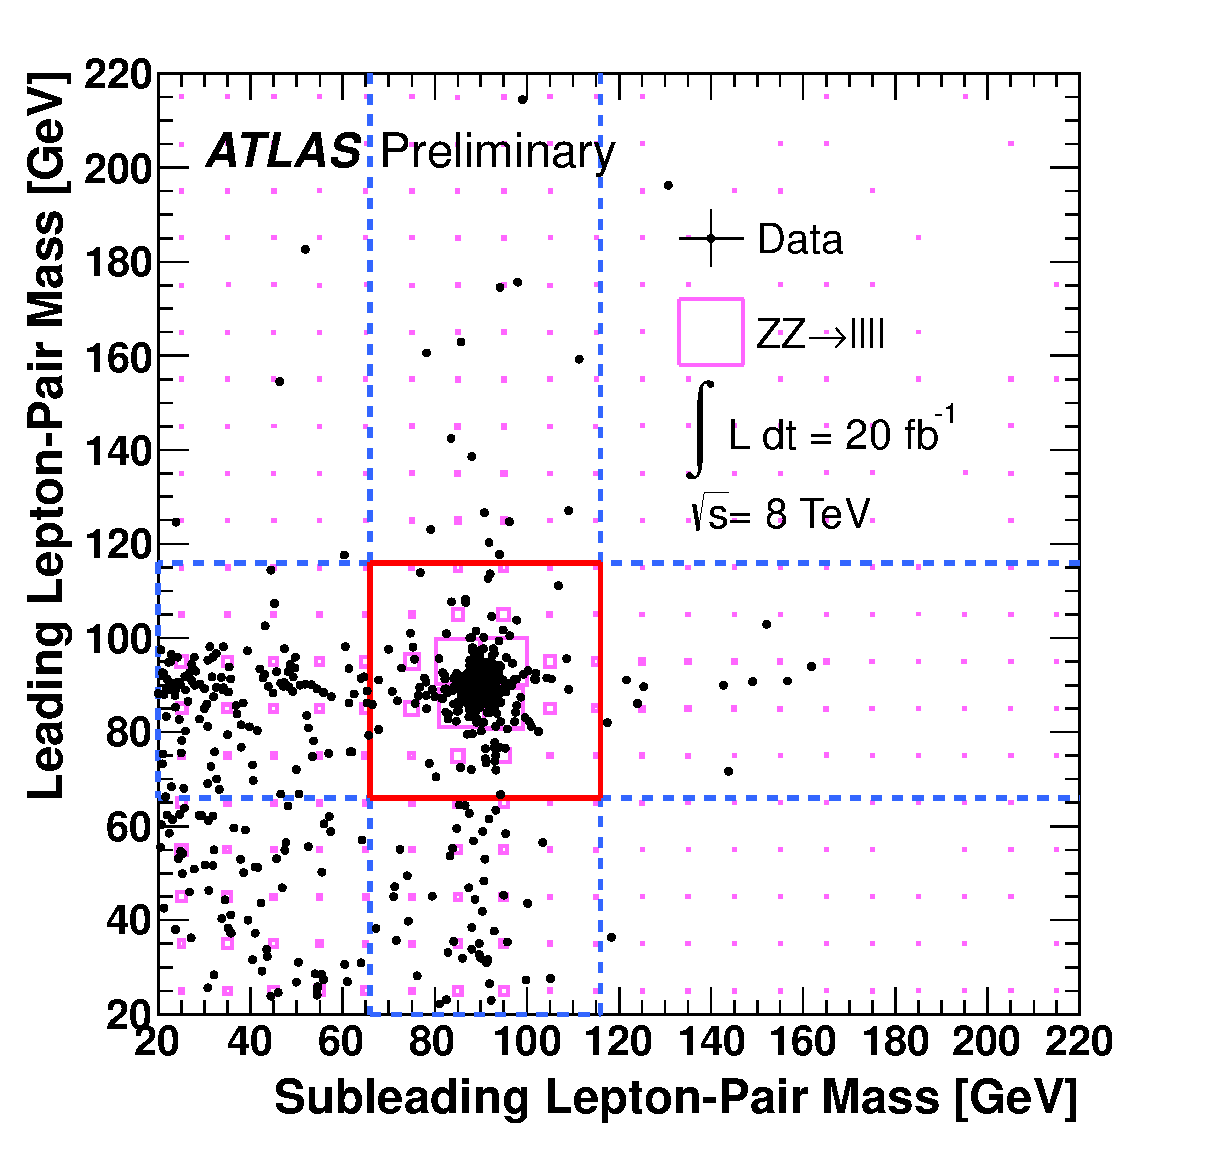
\includegraphics[width=0.9\textwidth]{8TeV/h_mz1_mz2}\hfill
  \caption[Mass of the leading \leppair\ versus the mass of the
  sub-leading \leppair\ for candidate \ZZ\ events in the 8~\tev\ data.]
  {\small Mass of the leading \leppair\ versus the mass of the
  sub-leading \leppair for candidate \ZZ\ events in the 8~\tev\ data after
  applying all of the selection
  requirements apart from the \dilepton\ mass requirements.
  The events observed in the data are shown as solid circles and the \ZZsllll\
  signal prediction from simulation as boxes, with 
  the size of each box is proportional to the expected number of events in each bin.  
  The region enclosed by the solid (dashed) lines indicates the signal region defined by the
  \dilepton\ mass requirements for \ZZ\ (\ZZs) events.
  %The background estimate is described in section 5.1.
   }
    \label{fig:zzdists-Zmass2D-eight}
 \end{center}
 \end{figure}

% pT_Z vs dR 7 TeV
 \begin{figure}[htbp]
 \begin{center}
  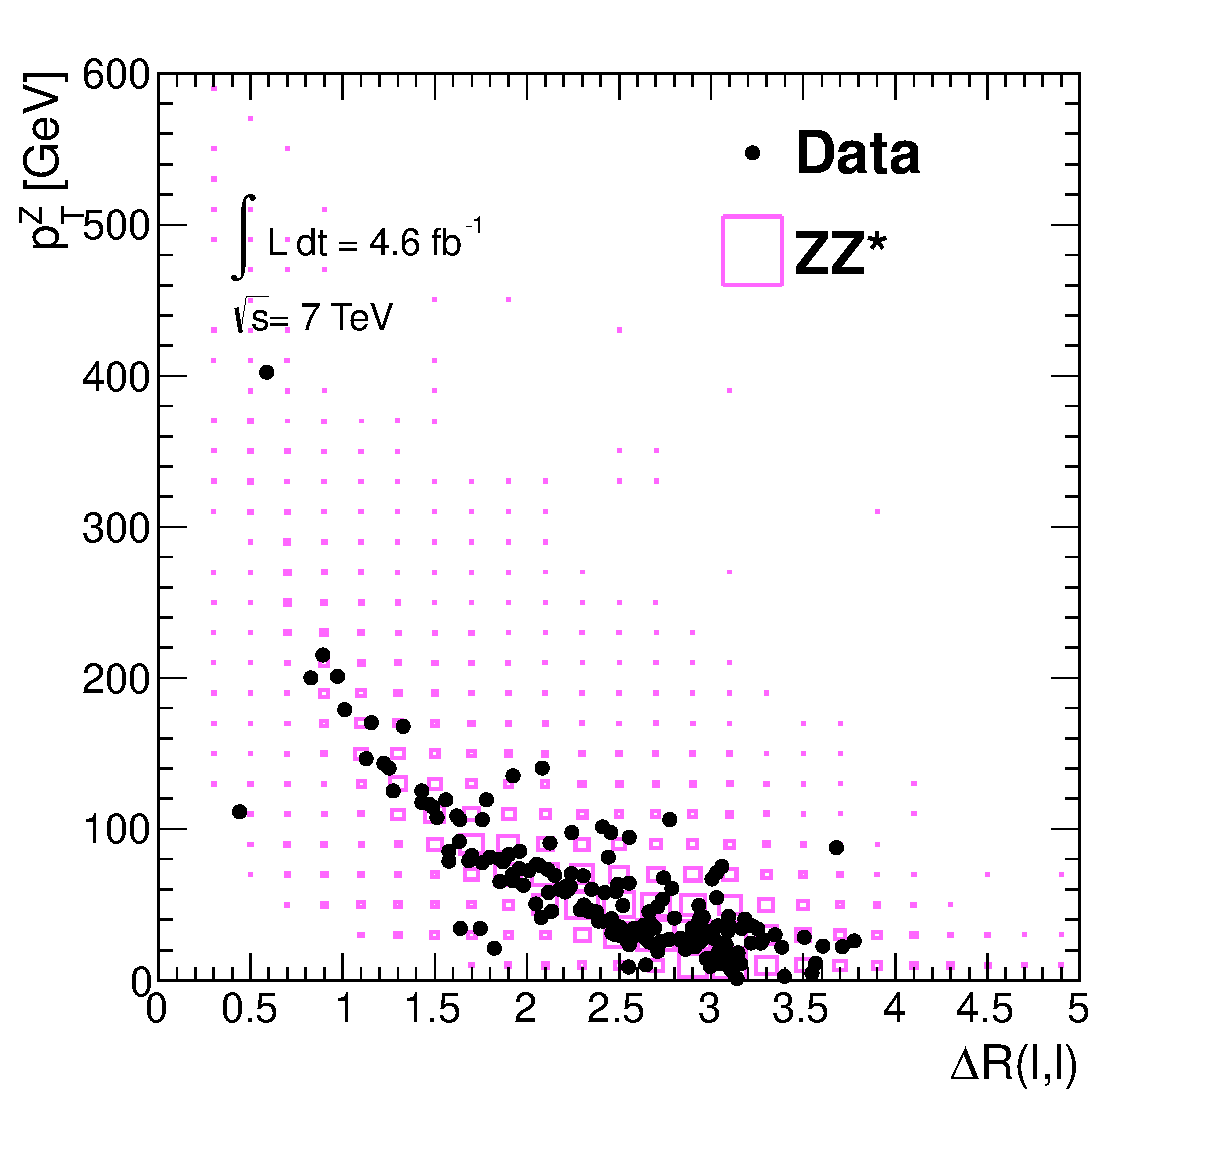
\includegraphics[width=0.7\textwidth]{7TeV/h_dr_ptz}\hfill
  \caption[Transverse momentum of \leppair s versus the opening angle between the leptons
    forming the pair, for events passing the \ZZs\ selection in 7~\tev\ data.]
    {\small Transverse momentum of  \leppair s versus the opening angle between the leptons
    forming the pair, for events passing the \ZZs\ selection in 7~\tev\ data (two
    entries per event).}
 \label{fig:zzdists-dr-ptz-seven}
 \end{center}
 \end{figure}

% m_ZZ vs min(dR) 7 TeV
% !! Not sure what this plot tells us - not much I suspect.
% \begin{figure}[htbp]
% \begin{center}
%  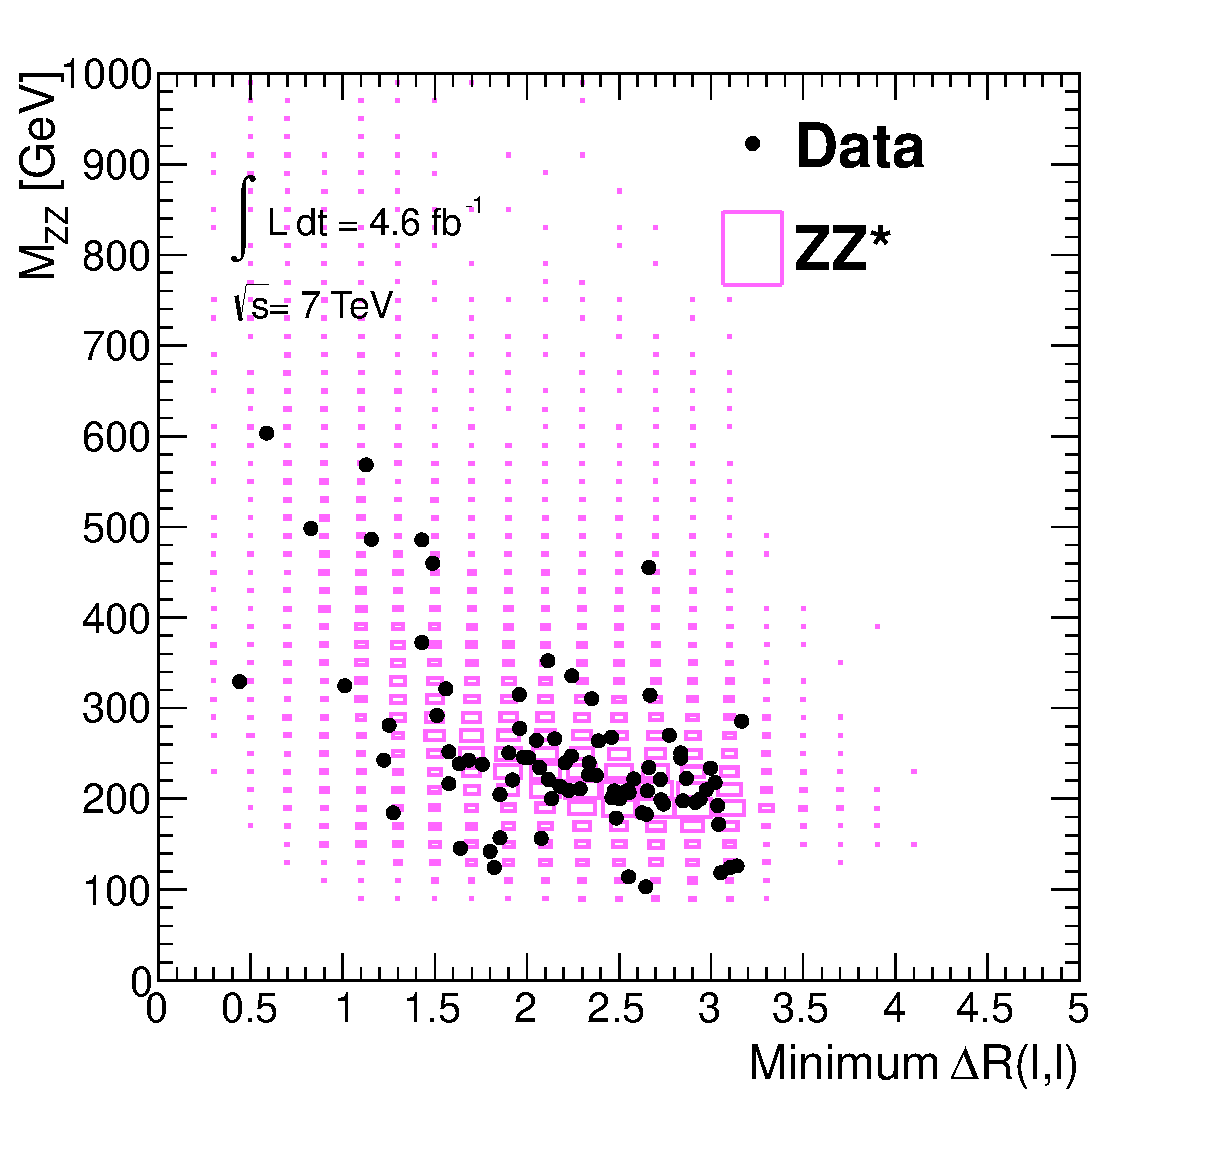
\includegraphics[width=0.7\textwidth]{7TeV/h_mindr_mzz}\hfill
%  \caption[The invariant mass of the four lepton system \mZZp\ versus the
%    minimum \deltaR\ between any pair of leptons in the event for events passing
%    the \ZZs\ selection in 7~\tev\ data.]
%    {\small The invariant mass of the four lepton system \mZZp\ versus the
%    minimum \deltaR\ between any pair of leptons in the event for events passing
%    the \ZZs\ selection in 7~\tev\ data.
%    The events observed in the data are shown as black dots and the signal prediction as boxes.}
% \label{fig:zzdists-mindr-mzz-seven}
% \end{center}
% \end{figure}

% 7 TeV, Z1_m, Z2_m, m_Z>7GeV
\begin{figure}[htbp]
    \begin{center}
     \subfigure[]{
     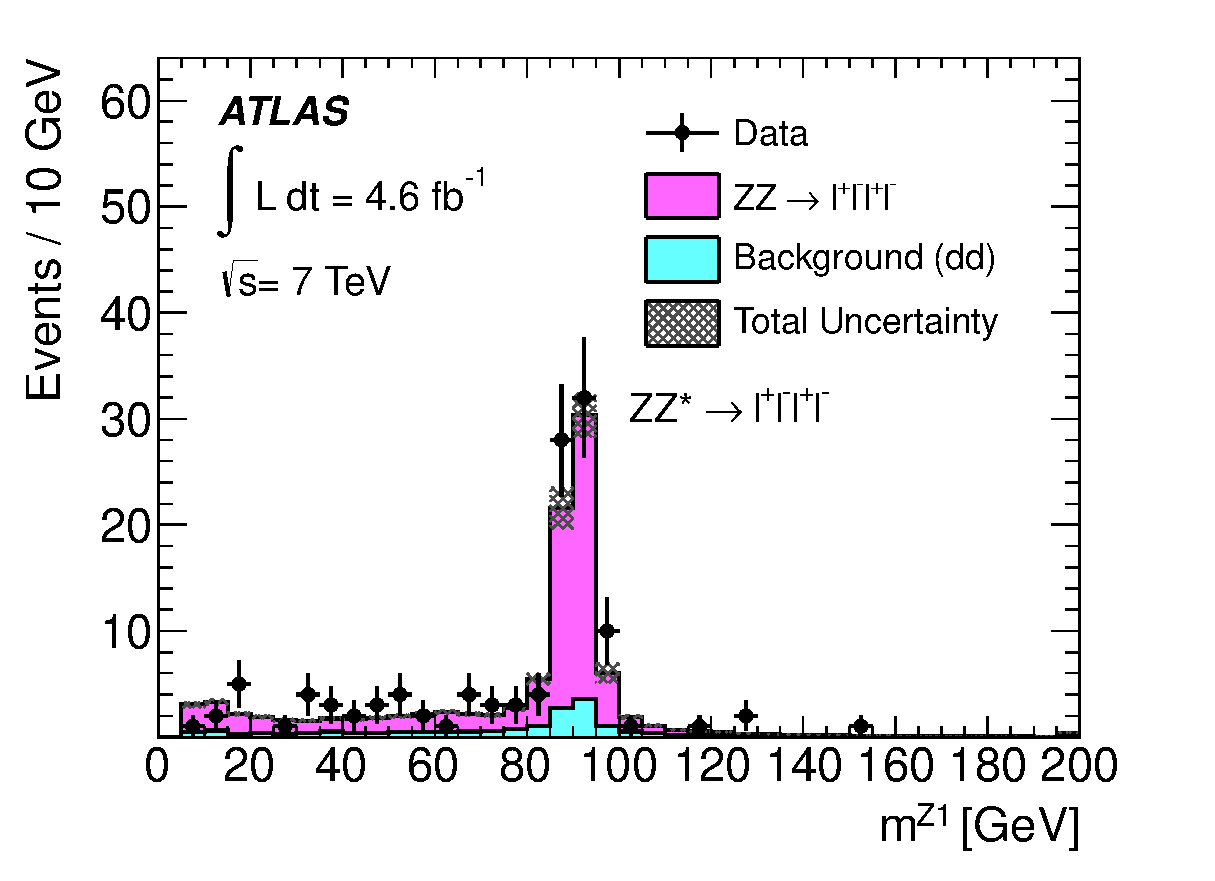
\includegraphics[width=0.47\textwidth]{7TeV/h_4l_ZZs_Z1_m}
     }
     \subfigure[]{
     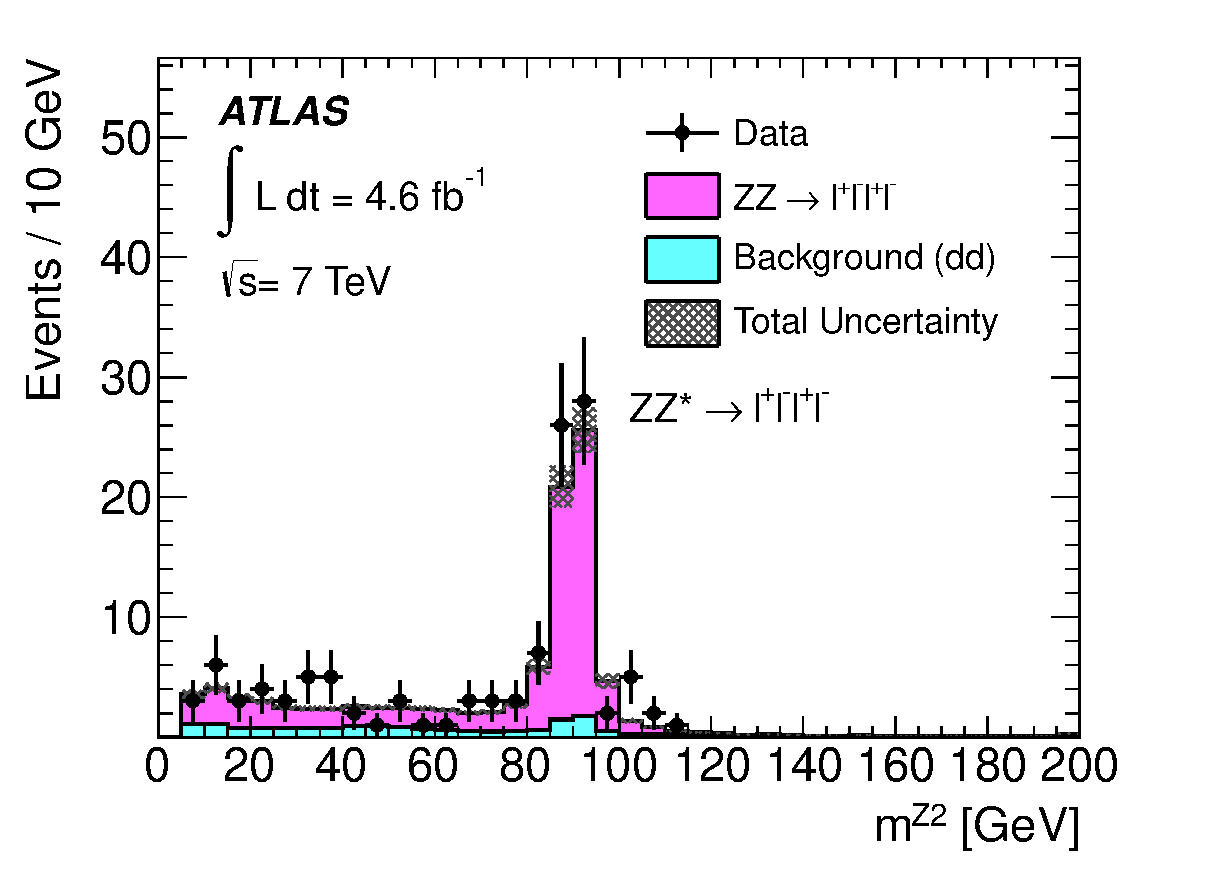
\includegraphics[width=0.47\textwidth]{7TeV/h_4l_ZZs_Z2_m}
     }
    \caption[Invariant masses of the leading and subleading \leppair\
    in candidate \ZZ\ events in the 7~\tev\ data.]
    {Invariant masses of the (a) leading and (b) subleading \leppair\ in
    candidate \ZZ\ events in the 7~\tev\ data. In each plot, the \leppair\
    not shown in the plot is required to pass the \sstooos\
    requirement. The points represent the observed data and the histograms show
    the prediction from simulation, where the background is normalised to the
    total background estimate as described in~\chap{BackgroundEstimate}.  The
    shaded band shows the combined statistical and systematic uncertainty on the
    prediction. 
}
    \label{fig:zzdists-Zmass-seven}
\end{center}
\end{figure}

% 8 TeV, Z1_m, Z2_m, m_Z>7GeV
\begin{figure}[htbp]
    \begin{center}
     \subfigure[]{
     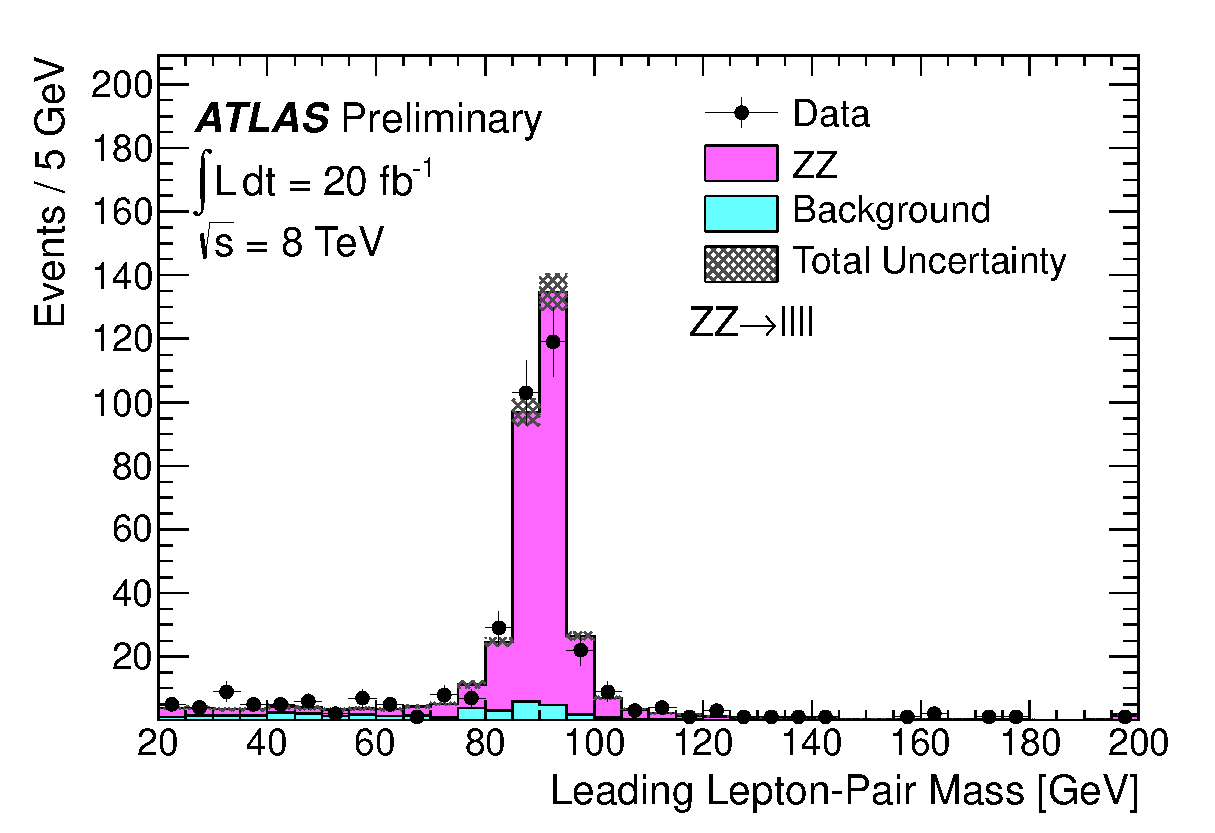
\includegraphics[width=0.47\textwidth]{8TeV/Z1_m_nm1_4l}
     }
     \subfigure[]{
     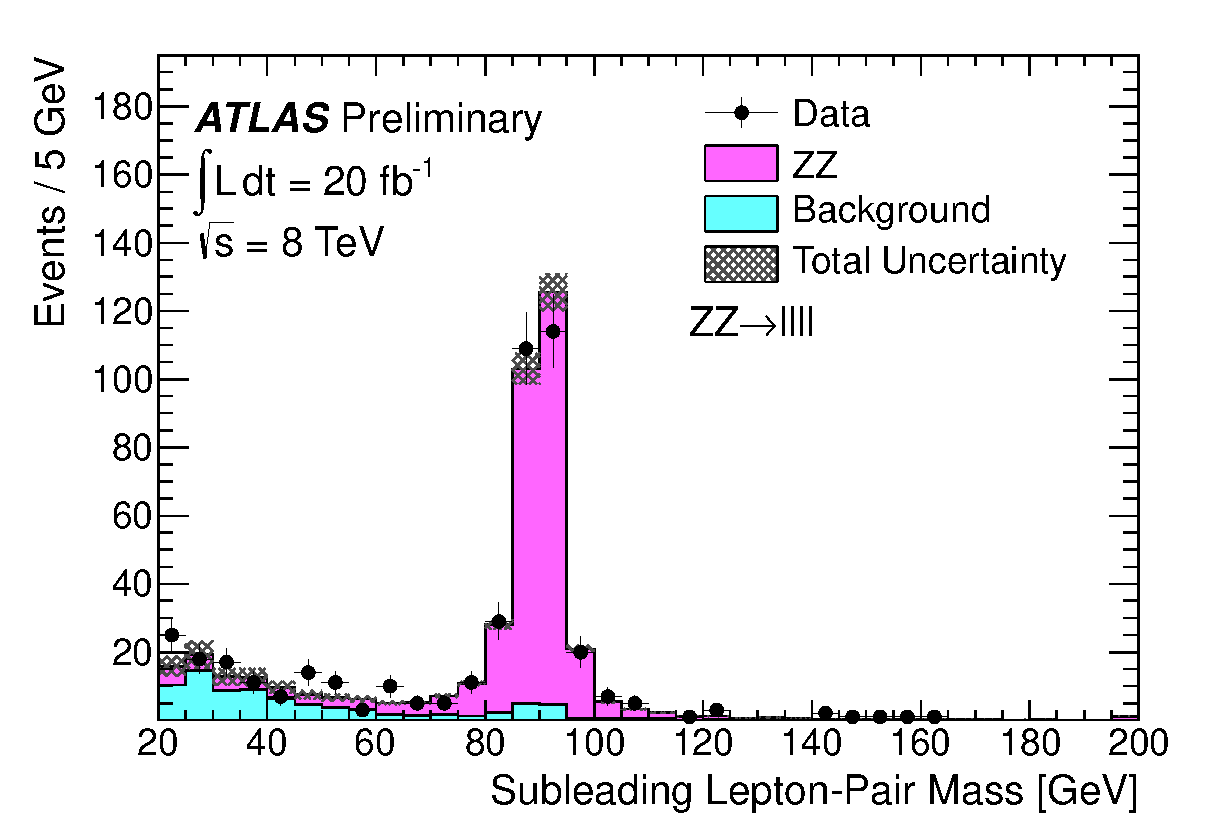
\includegraphics[width=0.47\textwidth]{8TeV/Z2_m_nm1_4l}
     }
    \caption[Invariant masses of the leading and subleading \leppair\
    in candidate \ZZ\ events in the 8~\tev\ data.]
    {Invariant masses of the (a) leading and (b) subleading \leppair\ in
    candidate \ZZ\ events in the 8~\tev\ data.  In each plot, the \leppair\    
    not shown in the plot is required to pass the \sstooos\
    requirement.  The points represent the observed data and the pink histogram
    shows the prediction for the signal from simulation. The light blue
    histogram shows the background shape obtained from data, normalised to the
    total background estimate as described in~\chap{BackgroundEstimate}.  The
    shaded band shows the combined statistical and systematic uncertainty on the
    prediction. 
}
    \label{fig:zzdists-Zmass-eight}
\end{center}
\end{figure}

% 7 TeV, ZZ, ZZ_pt / ZZ_m
\begin{figure}[htbp]
    \begin{center}
     \subfigure[]{
     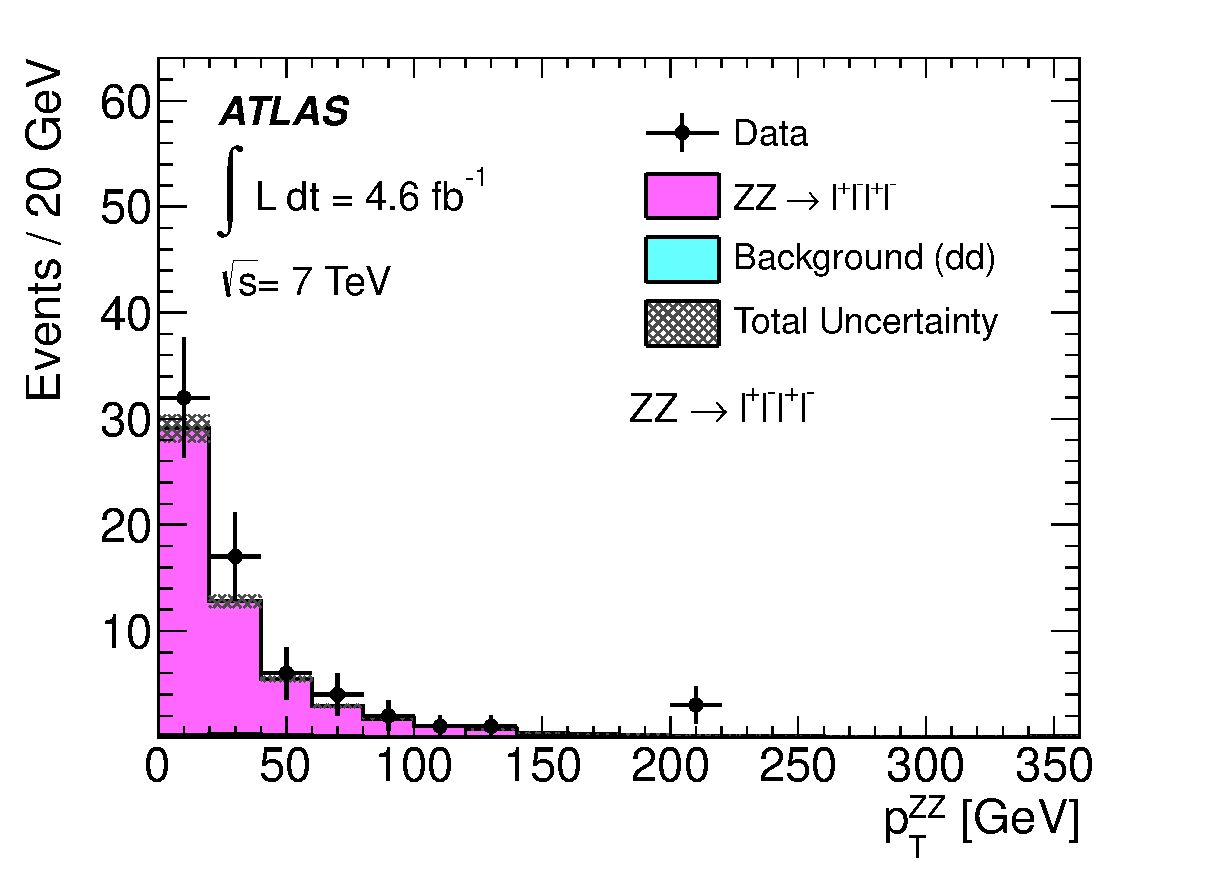
\includegraphics[width=0.47\textwidth]{7TeV/h_4l_ZZ_ZZ_pt}
     }
     \subfigure[]{
     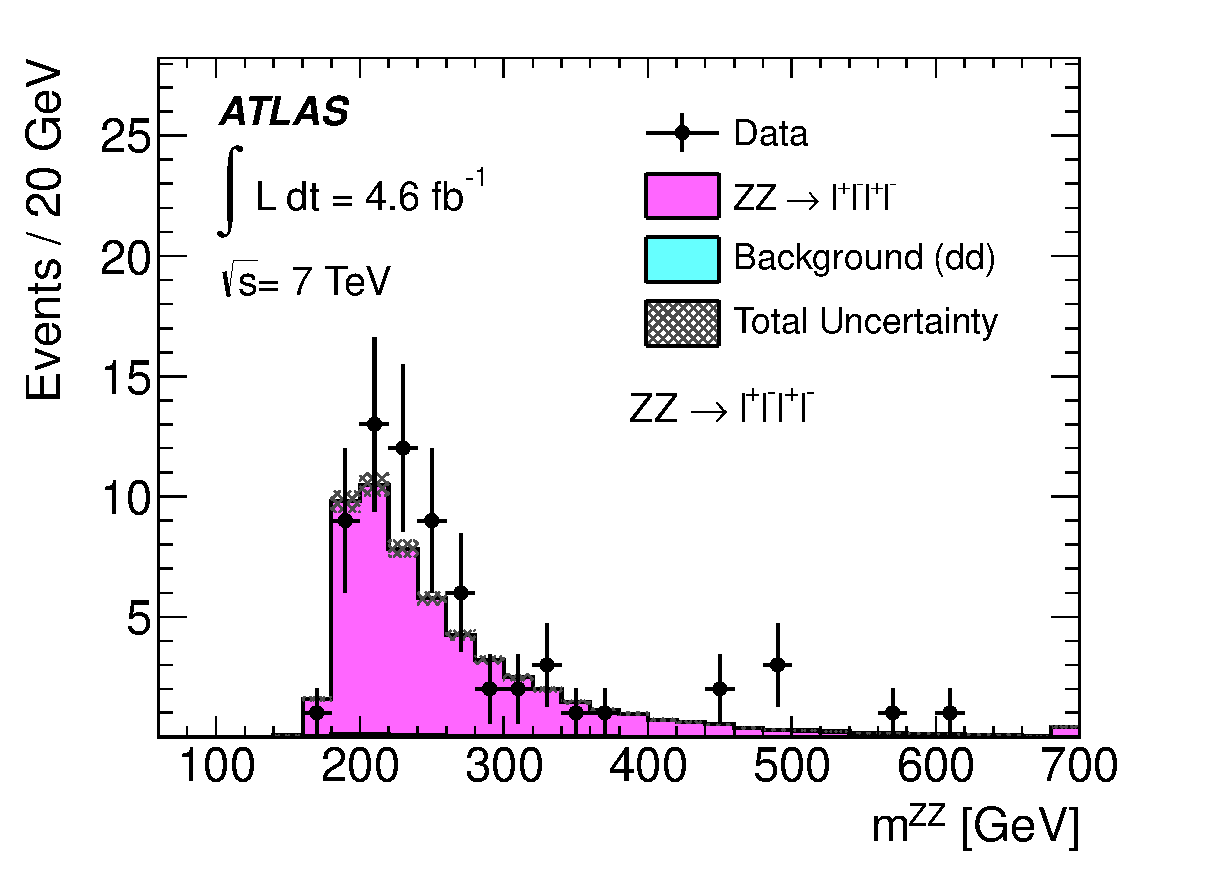
\includegraphics[width=0.47\textwidth]{7TeV/h_4l_ZZ_ZZ_m}
     }
     \subfigure[]{
     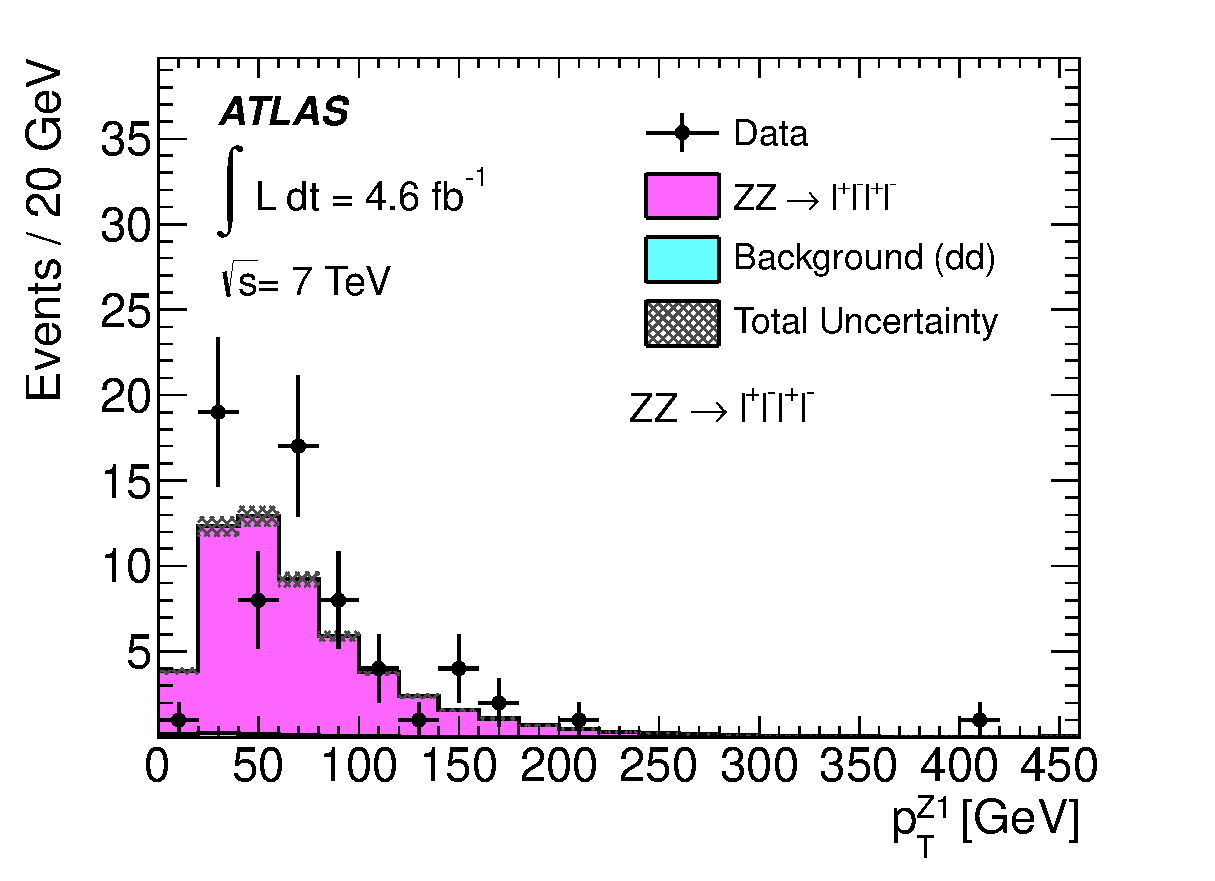
\includegraphics[width=0.47\textwidth]{7TeV/h_4l_ZZ_Z1_pt}
     }
     \subfigure[]{
     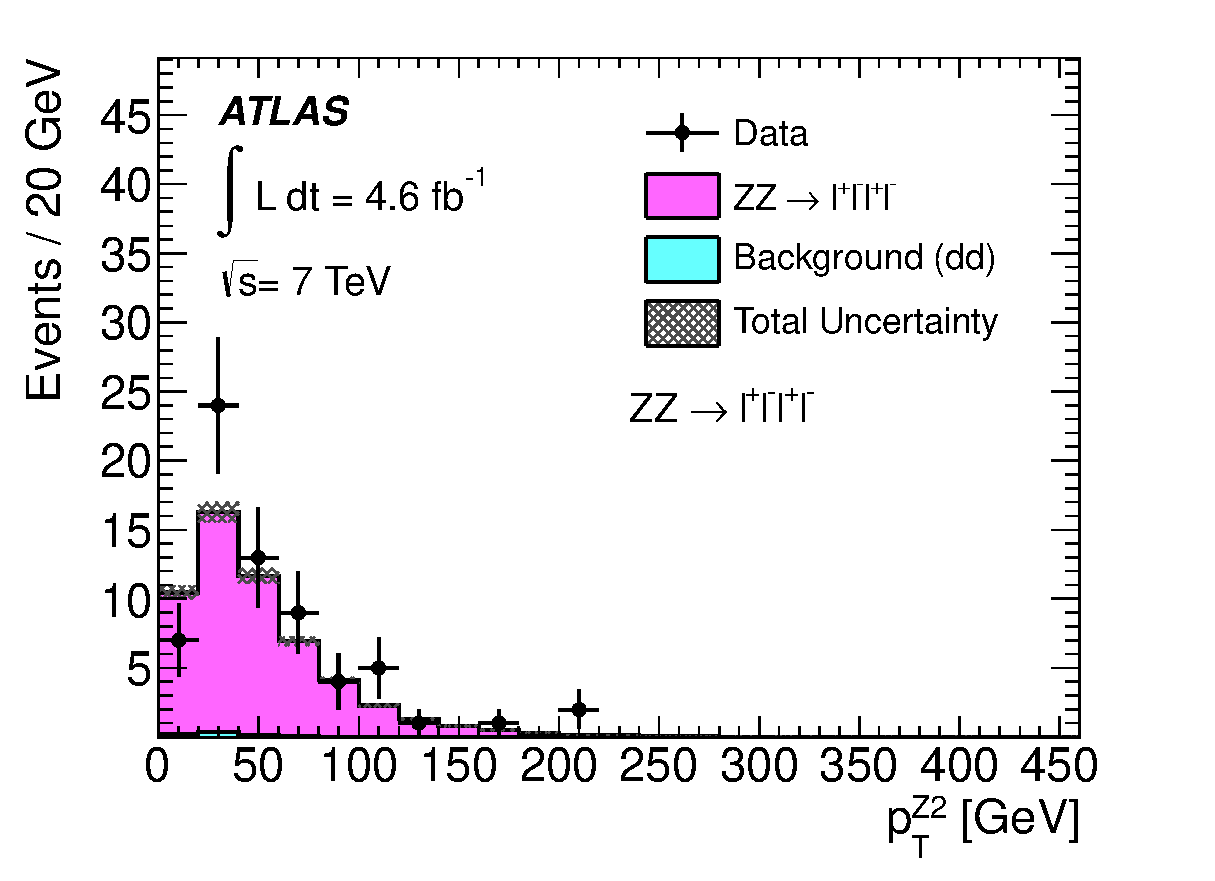
\includegraphics[width=0.47\textwidth]{7TeV/h_4l_ZZ_Z2_pt}
     }
    \caption[Kinematic distributions for events passing the \ZZ\ selection in
    the 7~\tev\ data.]
    {Kinematic distributions for events passing the \ZZ\ selection in
    the 7~\tev\ data: (a) transverse momentum $\pT^{\ZZ}$ and (b) invariant mass $m^{\ZZ}$ of the 
    four-lepton system, (c) transverse momentum of the leading
    \dilep\ pair $\pt^{Z1}$, and (d) transverse momentum of the subleading
    \dilep\ pair $\pt^{Z2}$. The points represent the observed data and the 
    histograms show the prediction from simulation, where the background
    is normalised to the total background estimate as described in
    ~\chap{BackgroundEstimate}. The shaded band 
    shows the combined statistical and systematic uncertainty on the prediction. 
    }
    \label{fig:zzdists-ZZ-seven}
    \end{center}
\end{figure}

% 8 TeV, ZZ, ZZ_pt / ZZ_m
\begin{figure}[htbp]
    \begin{center}
     \subfigure[]{
     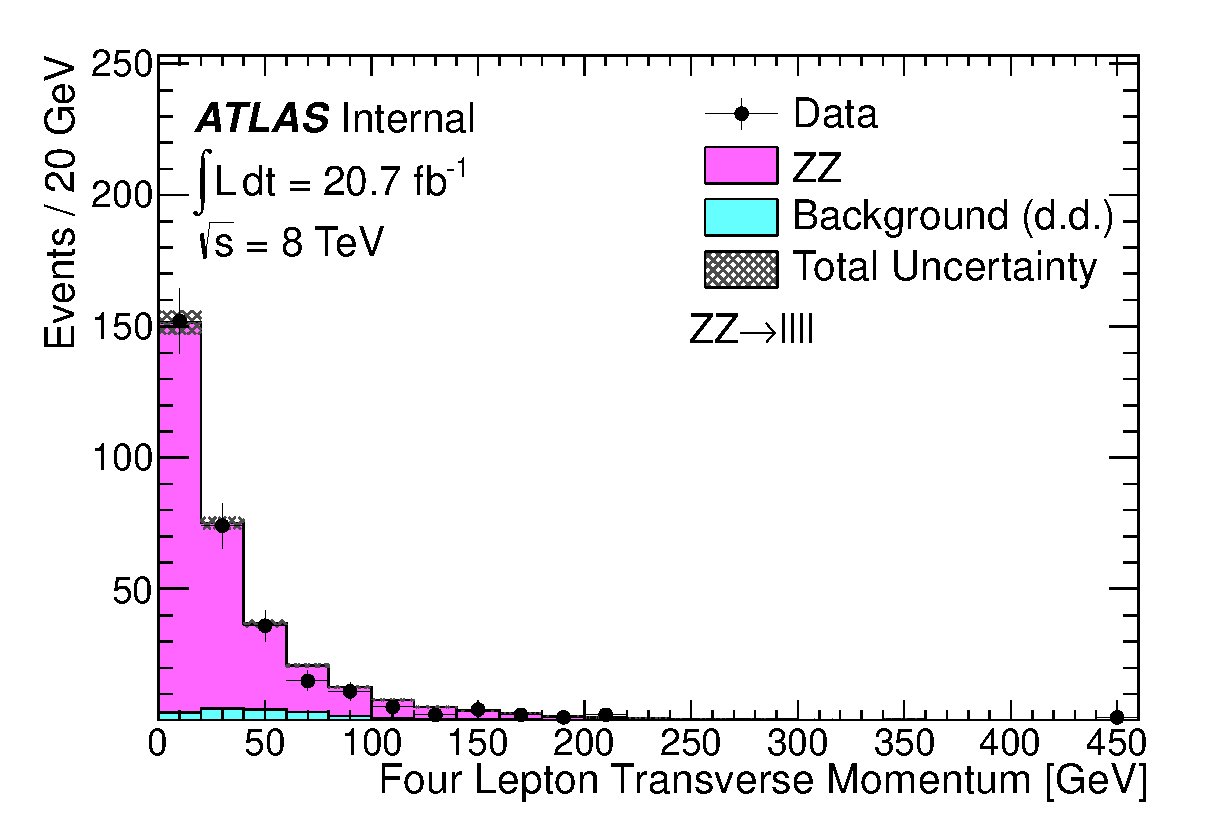
\includegraphics[width=0.47\textwidth]{8TeV/zzPt}
     }
     \subfigure[]{
     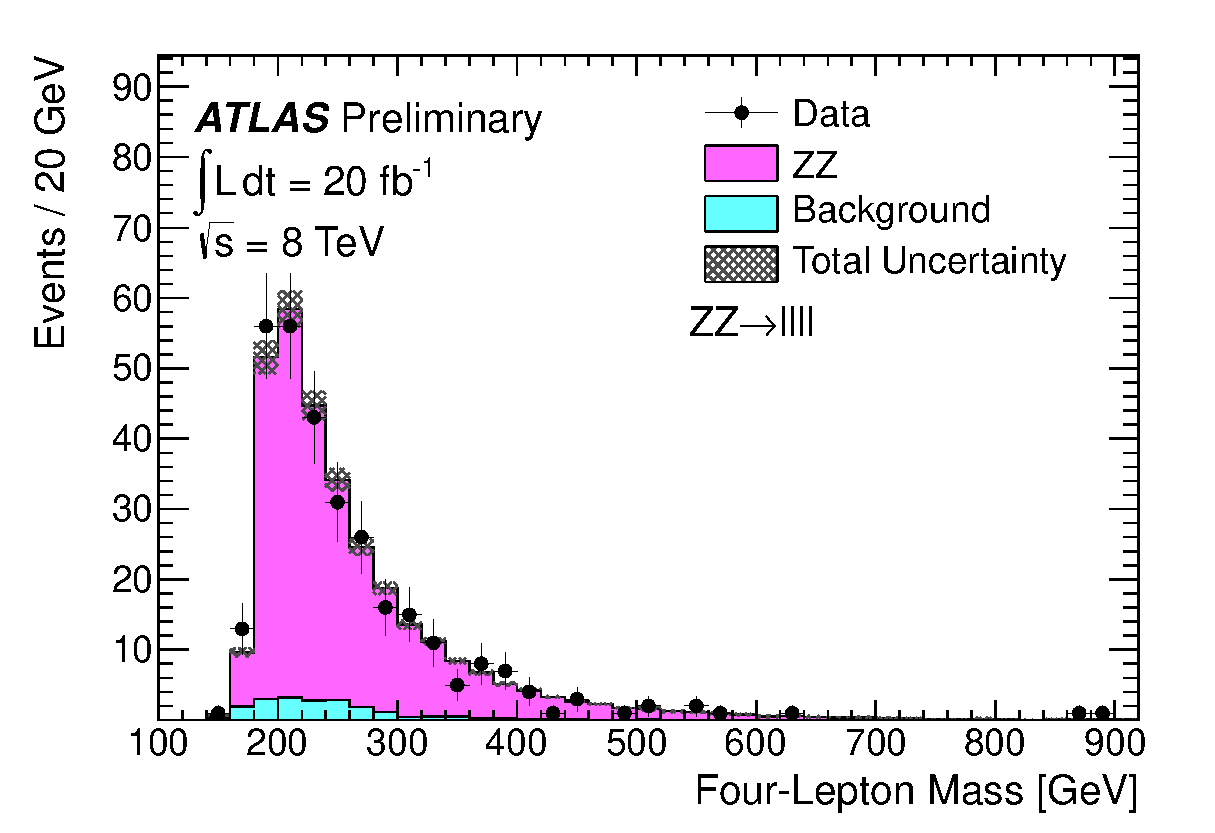
\includegraphics[width=0.47\textwidth]{8TeV/M4l}
     }
     \subfigure[]{
     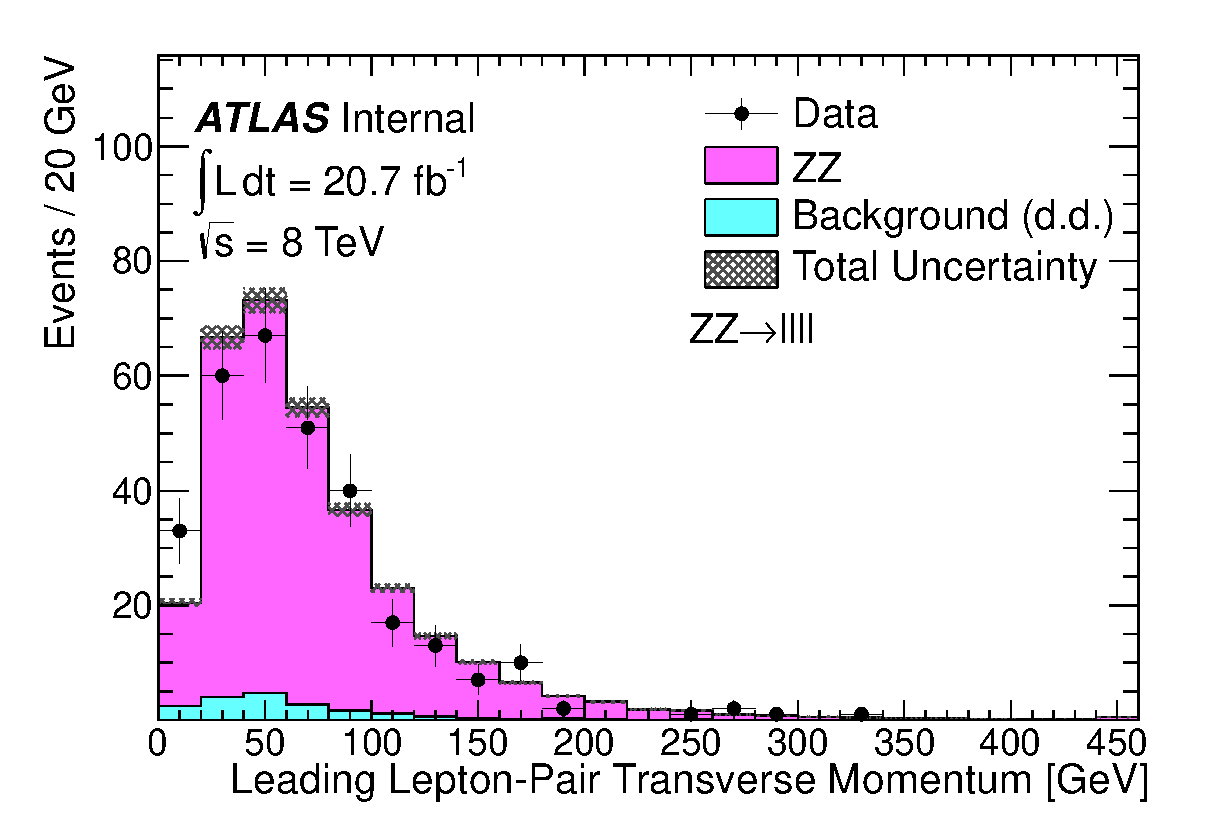
\includegraphics[width=0.47\textwidth]{8TeV/z1Pt}
     }
     \subfigure[]{
     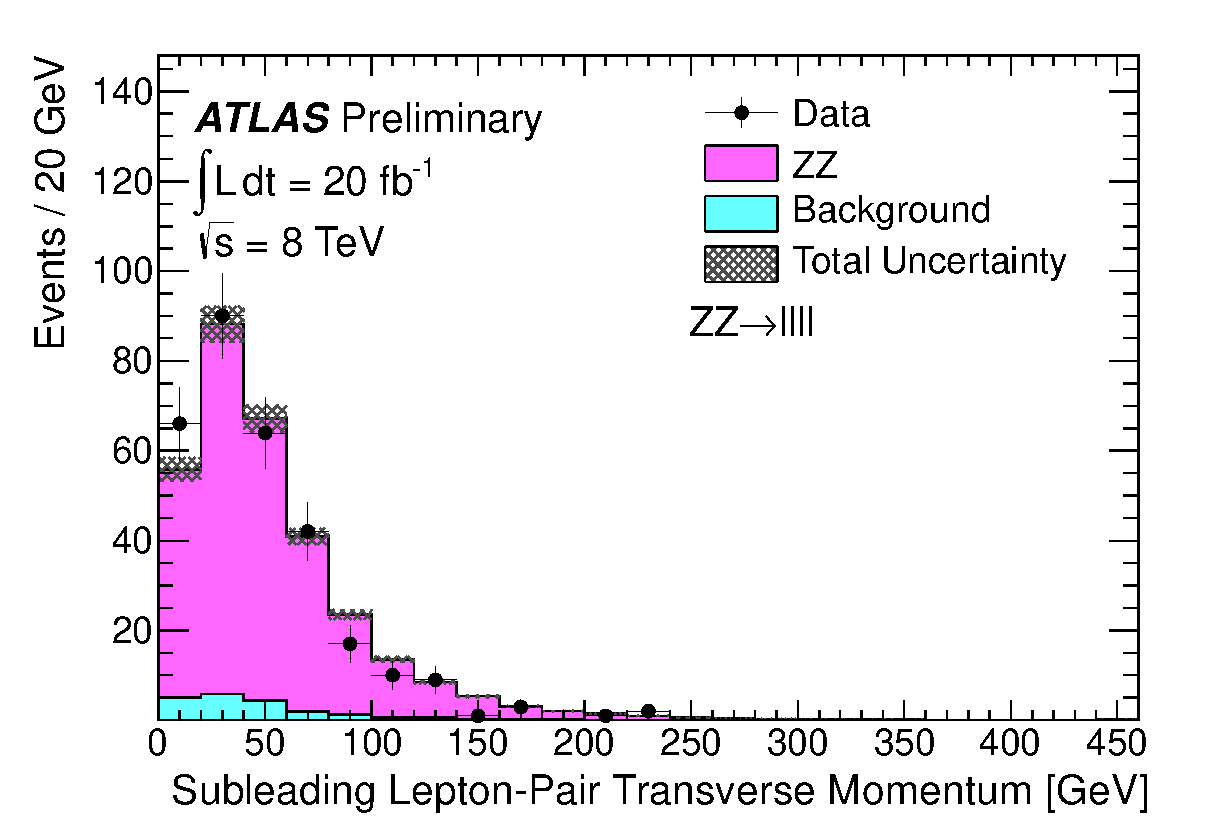
\includegraphics[width=0.47\textwidth]{8TeV/z2Pt}
     }
    \caption[Kinematic distributions for events passing the \ZZ\ selection in
    the 8~\tev\ data.]
    {Kinematic distributions for events passing the \ZZ\ selection in
    the 8~\tev\ data: (a) transverse momentum $\pT^{\ZZ}$ and (b) invariant mass $m^{\ZZ}$ of the 
    four-lepton system, (c) transverse momentum of the leading
    \dilep\ pair $\pt^{Z1}$, and (d) transverse momentum of the subleading
    \dilep\ pair $\pt^{Z2}$. The points represent the observed data and the pink histogram
    shows the prediction for the signal from simulation. The light blue
    histogram shows the background shape obtained from data, normalised to the
    total background estimate as described in~\chap{BackgroundEstimate}. The shaded band 
    shows the combined statistical and systematic uncertainty on the prediction. 
    }
    \label{fig:zzdists-ZZ-eight}
    \end{center}
\end{figure}
% 7 TeV, ZZ*, ZZ_pt / ZZ_m
\begin{figure}[htbp]
\begin{center}
    \subfigure[]{
    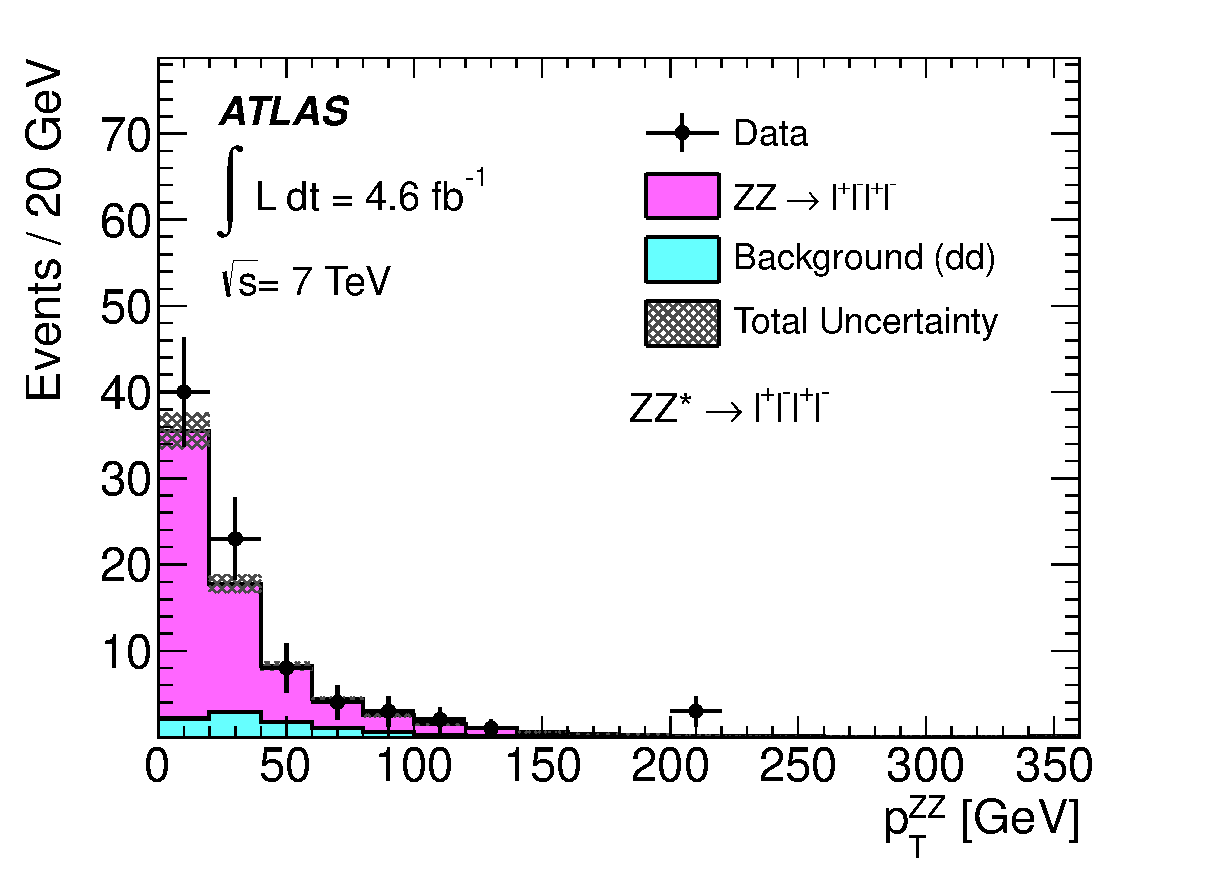
\includegraphics[width=0.47\textwidth]{7TeV/h_4l_ZZs_ZZ_pt}
    }
    \subfigure[]{
    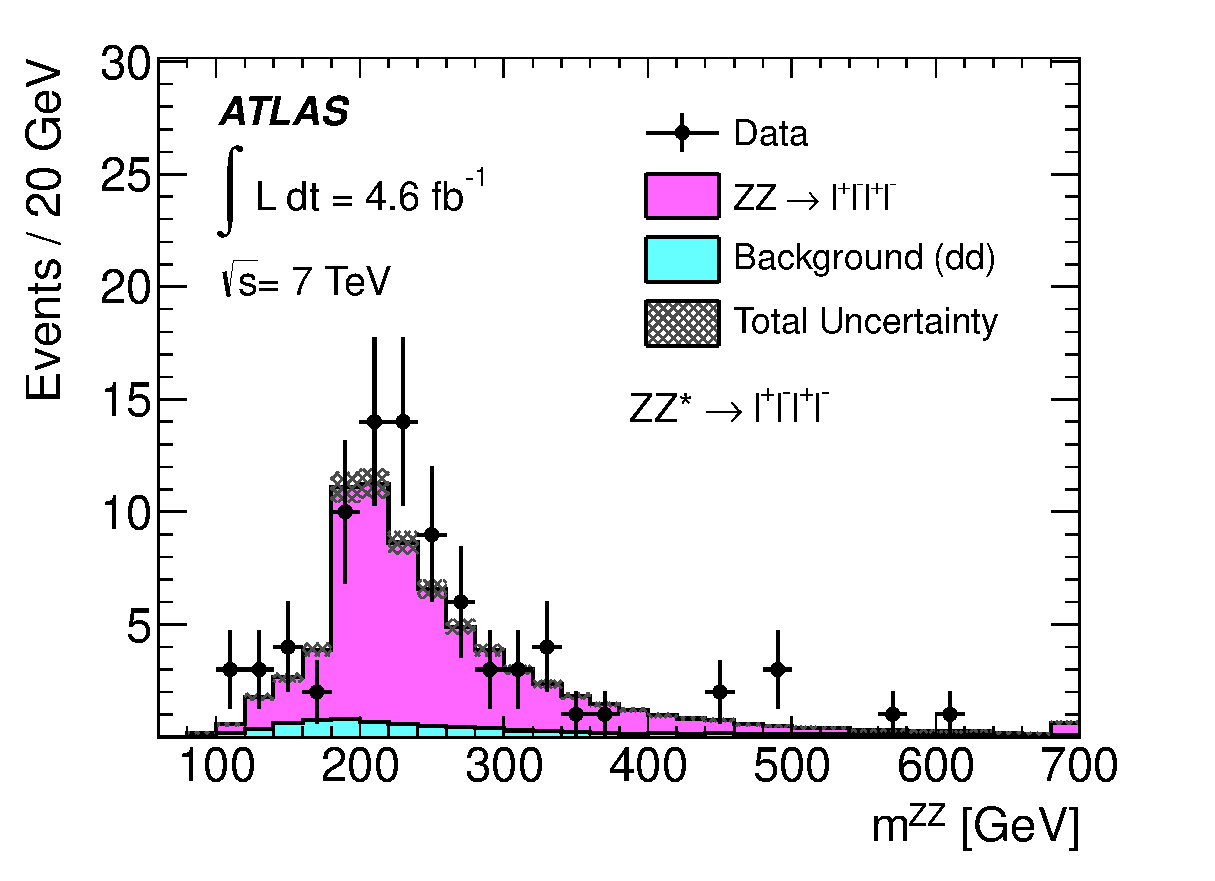
\includegraphics[width=0.47\textwidth]{7TeV/h_4l_ZZs_ZZ_m}
    }
    \subfigure[]{
    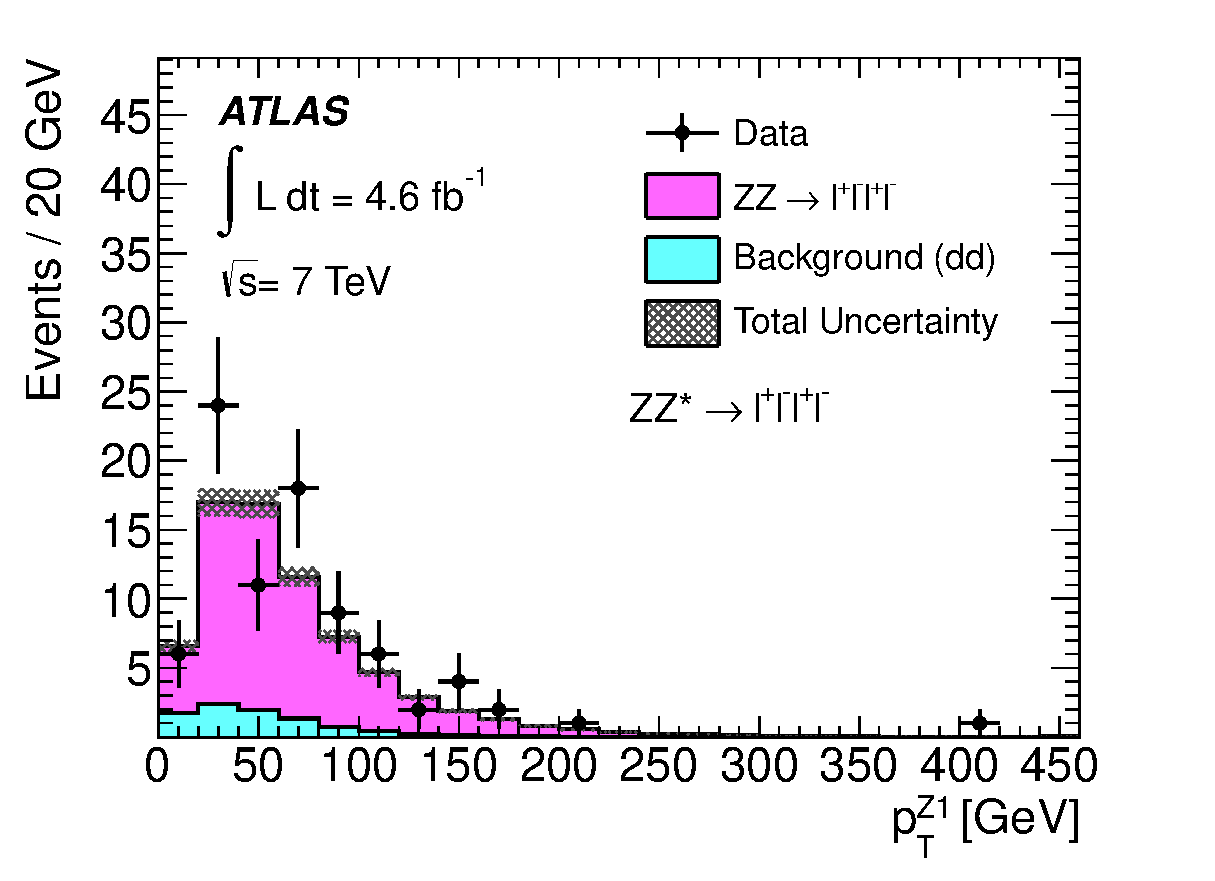
\includegraphics[width=0.47\textwidth]{7TeV/h_4l_ZZs_Z1_pt}
    }
    \subfigure[]{
    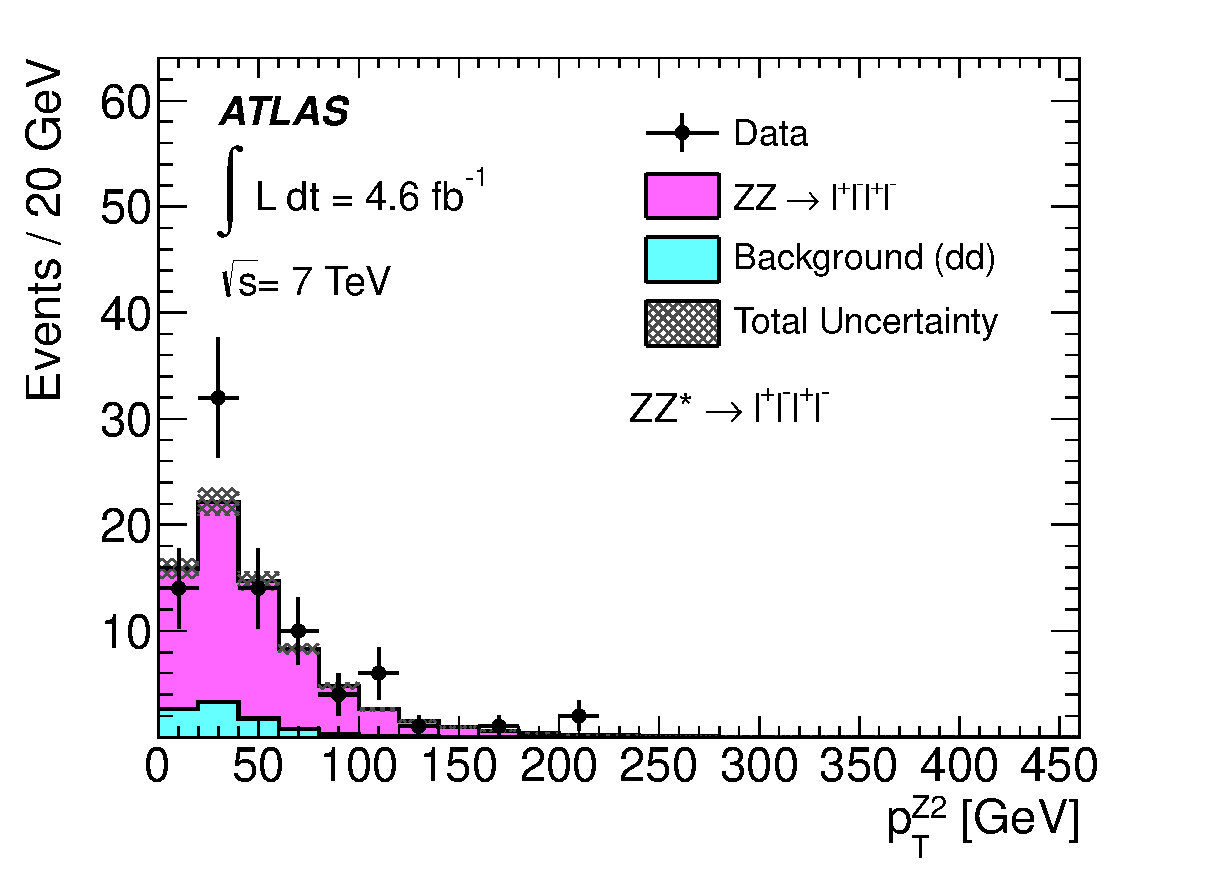
\includegraphics[width=0.47\textwidth]{7TeV/h_4l_ZZs_Z2_pt}
    }
    \caption[Kinematic distributions for events passing the \ZZs\ selection in
    the 7~\tev\ data.]
    {Kinematic distributions for events passing the \ZZs\ selection in
    the 7~\tev\ data: (a) transverse momentum $\pT^{\ZZ}$ and (b) invariant mass $m^{\ZZ}$ of the 
    four-lepton system, (c) transverse momentum of the leading
    \dilep\ pair $\pt^{Z1}$, and (d) transverse momentum of the subleading
    \dilep\ pair $\pt^{Z2}$. The points represent the observed data and the 
    histograms show the prediction from simulation, where the background
    is normalised to the data-driven estimate as described in
    ~\chap{BackgroundEstimate}. The shaded band 
    shows the combined statistical and systematic uncertainty on the prediction. 
    }
    \label{fig:zzdists-ZZs-seven}
\end{center}
\end{figure}


%% 8 TeV, ZZ*, ZZ_pt / ZZ_m
%\begin{figure}[htbp]
%\begin{center}
%    \subfigure[]{
%    
\includegraphics[width=0.47\textwidth]{placeholder}
%    }
%    \subfigure[]{
%    
\includegraphics[width=0.47\textwidth]{placeholder}
%    }
%    \subfigure[]{
%    
\includegraphics[width=0.47\textwidth]{placeholder}
%    }
%    \subfigure[]{
%    
\includegraphics[width=0.47\textwidth]{placeholder}
%    }
%    \caption[Kinematic distributions for events passing the \ZZs\ selection in
%    the 8~\tev\ data.]
%    {Kinematic distributions for events passing the \ZZs\ selection in
%    the 8~\tev\ data: (a) transverse momentum $\pT^{\ZZ}$ and (b) invariant mass $m^{\ZZ}$ of the 
%    four-lepton system, (c) transverse momentum of the leading
%    \dilep\ pair $\pt^{Z1}$, and (d) transverse momentum of the subleading
%    \dilep\ pair $\pt^{Z2}$. The points represent the observed data and the 
%    histograms show the prediction from simulation, where the background
%    is normalised to the data-driven (dd) estimate as described in
%    ~\chap{BackgroundEstimate}. The shaded band 
%    shows the combined statistical and systematic uncertainty on the prediction. 
%    }
%\end{center}
%    \label{fig:zzdists-ZZs-eight}
%\end{figure}

\section{\CX\ Measurement}

As discussed in~\sec{TheoryZZProduction-CxDef}, the \cx\ is first measured in a
fiducial \phasespace\
corresponding to the experimental selections (the \intro{fiducial \cx}), in
order to reduce systematic uncertainties associated with extrapolation. The
fiducial \cx\ is then extrapolated to the total \ZZ\ \cx, correcting for the
acceptance of the fiducial \phasespace\ and the \ZZlllplp\ branching fraction.  The definition of the
fiducial \phasespace\ was given in~\sec{TheoryZZProduction-CxDef}, and is slightly different for the
7~\tev\ and 8~\tev\ analyses due to the differing experimental selections.

\subsection{Fiducial \CX}

For a given \ZZllll\ final state the fiducial \cx\ is defined as:

\begin{equation}\label{eq:xsecfid_fourl}
\sigmaFidZZlllplp = \frac{\NObslllplp - \NBglllplp}{\mathcal{L} \times \CZZ^{\lllplp}}
\end{equation}
where \NObslllplp\ is  the number of observed event and \NBglllplp\ is the expected number
of background events. $\mathcal{L}$ is the integrated luminosity
of the data sample and
$\CZZ^{\lllplp}$ is the reconstruction acceptance factor for the \lllplp\
final-state, as defined in~\sec{objSel-CZZ}.

The \cx\ is estimated using a maximum profile-likelihood technique, by
maximising the \intro{profile-likelihood function, \L} with respect to the \cx\
$\sigma$.
\L\ is the product of the Poisson probability $P$ for observing $N$ events given a
\cx\ $\sigma$, reconstruction acceptance \CZZ\ and background $b$; and of Gaussian
distributions $G$ to describe nuisance parameters due to uncertainties on \CZZ,
$b$ and $\mathcal{L}$:

\begin{equation}
\begin{split}
%\small
   \L(\sigma, \CZZ', b'; \Delta_{b}, \Delta_{C_{ZZ}}, N) = P(\sigma, \CZZ^\prime,
   b^\prime; N)\times G(\CZZ^\prime; C_{ZZ}, \Delta_{C_{ZZ}}) \\
   \times G(b^\prime; b, \Delta_{b})
\times G(\mathcal{L}^\prime; \mathcal{L}, \Delta_{\mathcal{L}})
\end{split}
\end{equation}

The Poisson probability to observe $N$ events given an expected
number of signal events $s$ and expected background $b$ is:

\begin{equation}
P(\sigma, C_{ZZ}, b; N) =
\frac{e^{-(s+b)}\cdot
     \left(s+b\right)^{N}}
     {N!},
\end{equation}
where $s$ is given by:

\begin{equation}
   s(\sigmaFid, \CZZ, \mathcal{L}) = \sigmaFid\times\mathcal{L}\times\CZZ \\
\end{equation}

In practice, for computational convenience $-\ln(L)$ is minimised rather
than maximising $L$, however the procedures are equivalent. The fiducial
\cx\ for each final-state is calculated separately. For calculating the combined \ZZllll\
fiducial \cx, the number of observed and expected events for each individual
final-state are summed and the weighted average of the reconstruction
acceptances in each final-state is taken. 
%A combined background estimate is used,
%estimating the background for all \llll\ final states together; this benefits from a
%lower statistical uncertainty than simply summing the individual final-state background
%estimates. 
The background is estimated for all \llll\ final states combined (as in the last
column of~\tab{bg-est-final}); this benefits from a
lower statistical uncertainty than summing the individual final-state background
estimates. 
This procedure for combining the final-states gives the highest weight to the highest
statistics channels, and does not automatically take into account the better
signal over background ratios ($S/B$) in different final-states. However, since the
lowest statistics channel is also the channel with the worse $S/B$ (the \eeee\
final-state), this simpler approach is justified.

\subsubsection{Fiducial \CX\ Results}

Fiducial \cx\ results are presented in~\tab{meas-fid-cx}, together with the
theoretical predictions. For the 7~\tev\ analysis, the measured fiducial \cx s
are slightly higher than predicted by the theory, but are consistent within the
uncertainties.  For the 8~\tev\ analysis, the measured \cx s are in good
agreement with the theory.

%% Observed Fiducial Cross Sections, 7 TeV
\begin{table}
\renewcommand\arraystretch{1.3}
\centering
\small
  \begin{tabular}{lll}
    \hline\hline
     Channel & Measured Fiducial \CX   & Theory                              \\
     %7~\tev, \ZZ             &                          \\
    \hline
     {\bf \underline{7~\tev, \ZZ}}             &                          \\
     \ZZeeee\       & \ZZSevenTeVFiducialCrossSectionZZEEEE   & \ZZSevenTeVTheoryFiducialCrossSectionZZEEEE \\
     \ZZmmmm\       & \ZZSevenTeVFiducialCrossSectionZZMMMM   & \ZZSevenTeVTheoryFiducialCrossSectionZZMMMM \\
     \ZZeemm\       & \ZZSevenTeVFiducialCrossSectionZZEEMM   & \ZZSevenTeVTheoryFiducialCrossSectionZZEEMM \\
     \ZZllll\   & \ZZSevenTeVFiducialCrossSectionZZLLLL   & \ZZSevenTeVTheoryFiducialCrossSectionZZLLLL \\
    %\hline\hline
    %\\
    %\hline\hline
     %7~\tev, \ZZs             &                          \\
    \hline
     {\bf \underline{7~\tev, \ZZs}}             &                          \\
     \ZZseeee\      & \ZZSevenTeVFiducialCrossSectionZZsEEEE & \ZZSevenTeVTheoryFiducialCrossSectionZZsEEEE   \\
     \ZZsmmmm\      & \ZZSevenTeVFiducialCrossSectionZZsMMMM & \ZZSevenTeVTheoryFiducialCrossSectionZZsMMMM   \\
     \ZZseemm\      & \ZZSevenTeVFiducialCrossSectionZZsEEMM & \ZZSevenTeVTheoryFiducialCrossSectionZZsEEMM   \\
     \ZZsllll\      & \ZZSevenTeVFiducialCrossSectionZZsLLLL & \ZZSevenTeVTheoryFiducialCrossSectionZZsLLLL   \\
    \hline
     {\bf \underline{8~\tev, \ZZ}}             &                          \\
     \ZZeeee\       & \ZZEightTeVFiducialCrossSectionZZEEEE & \ZZEightTeVTheoryFiducialCrossSectionZZEEEE   \\
     \ZZmmmm\       & \ZZEightTeVFiducialCrossSectionZZMMMM & \ZZEightTeVTheoryFiducialCrossSectionZZMMMM   \\
     \ZZeemm\       & \ZZEightTeVFiducialCrossSectionZZEEMM & \ZZEightTeVTheoryFiducialCrossSectionZZEEMM   \\
     \ZZllll\       & \ZZEightTeVFiducialCrossSectionZZLLLL & \ZZEightTeVTheoryFiducialCrossSectionZZLLLL   \\
    \hline\hline
  \end{tabular}

      \caption[Fiducial \CX\ measurements at 7~\tev\ and at 8~\tev.]
      { Fiducial \CX\ measurements at 7~\tev\ and at 8~\tev. The second column
      gives the measured \cx, and the third the prediction from theory,
      calculated to NLO in QCD using MCFM 6.3 with PDF set CT10 and scale set to
      $\frac{1}{2}m(\ZZ)$. The quoted theoretical uncertainties are obtained by
      varying the factorisation and renormalisation scales, simultaneously, up
      and down by a
      factor of two, and by using the CT10 error set.} 
    \label{table:meas-fid-cx}
\renewcommand\arraystretch{1}
\end{table}

    %\calc{1+2}

\subsection{Total \CX}

The total \cx\ is obtained by extrapolating the fiducial \cx\ from the
fiducial \phasespace\ to the total \phasespace\ space and by correcting for the
\ZZllll\ branching fraction. The total \cx\ is defined by requiring both \Z\
bosons have mass \sstooosZ. In order to extrapolate from the fiducial to the
total \phasespace, the \intro{fiducial acceptance factor}, \AZZ, must be
estimated. \AZZ\ is the is fraction of \ZZ\ events with both \Z\ bosons passing
the \sstooosZ\ requirement which fall into the fiducial \phasespace, and is
estimated from \mcsim\ as:

\begin{equation}
\AZZ = \frac{ N^{\rm MC\ Fiducial\ Volume}_{{\rm Generated}\ ZZ} }{ N^{{\rm MC\
All}}_{{\rm Generated}\ ZZ} }
\end{equation}
The total \cx\ is then defined as:

\begin{equation}\label{eq:xsectot_fourl}
\sigmaTotZZ = \frac{ \NObs - \NBg}{\mathcal{L} \times
BR\{\ZZllll\} \times \AZZ \times \CZZ}
\end{equation}
Uncertainties on \AZZ\ arise due to uncertainties on the \partDF, the choice of
the factorisation and renormalisation scales and modelling of the parton shower
and ISR. \AZZ\ is determined using the \powhegbox\ and \ggtwoZZ\ generators. The
PDF errors are estimated using the 52 CT10 error sets and by taking the
difference with MSTW2008, and the scale errors are estimated by varying the
factorisation and renormalisation scales, simultaneously, 
up and down by a factor of two. The systematic due to the modelling of the parton shower
and ISR is estimated by comparing the value for \AZZ\ obtained from a
\powhegbox\ sample showered with \herwig\ compared to to the nominal sample
which is showered with \pythia. Additionally, the difference with the \AZZ\
obtained from MCFM, which does not model the parton shower, is taken as an
additional systematic. The contributions of these different sources of
systematic uncertainty are shown in~\tab{azz-syst}, and the values of \AZZ\ are
shown in~\tab{azz}. The \AZZ\ are smaller for the 8~\tev\ analysis reflecting the tighter lepton $\eta$ 
requirement in the definition of the fiducial \phasespace\ at 8~\tev\ with
respect to 7~\tev.
% 1.1 % quoted in note seems to be difference between having showering and not,
% ie MCFM vs Powheg

\begin{table}
\renewcommand\arraystretch{1.1}
\centering
\small
  \begin{tabular}{lll}
    \hline\hline
     Source (\%) & 7~\tev & 8~\tev \\
    \hline
     PDF  & \ZZSevenTeVAZZPDFUncPercentage\ & \ZZEightTeVAZZPDFUncPercentage \\
     Scale  & \ZZSevenTeVAZZScaleUncPercentage\ & \ZZEightTeVAZZScaleUncPercentage \\
     Parton Shower / ISR Model  & \ZZSevenTeVAZZISRUncPercentage\ & \ZZEightTeVAZZISRUncPercentage \\
     Generator Difference  & \ZZSevenTeVAZZGenUncPercentage\ & \ZZEightTeVAZZGenUncPercentage \\
     \hline
     Total  & \ZZSevenTeVAZZTotalUncPercentage\ & \ZZEightTeVAZZTotalUncPercentage \\
    \hline\hline
  \end{tabular}

      \caption[Systematic uncertainties to the fiducial acceptance factors, \AZZ, at 7~\tev\ and at 8~\tev.]
      { Systematic uncertainties to the fiducial acceptance factors, \AZZ, at
      7~\tev\ and at 8~\tev. }
    \label{table:azz-syst}
\renewcommand\arraystretch{1}
\end{table}


\begin{table}
\renewcommand\arraystretch{1.1}
\centering
\small
  \begin{tabular}{lll}
    \hline\hline
     Channel & 7~\tev & 8~\tev \\
    \hline
     \ZZeeee\       &
     \measSyst{\ZZSevenTeVAZZCentral}{\errSym{\ZZSevenTeVAZZSystUnc}}   & 
     \measSyst{\ZZEightTeVAZZCentral}{\errSym{\ZZEightTeVAZZSystUnc}}   \\
     \ZZmmmm\       &
     \measSyst{\ZZSevenTeVAZZCentral}{\errSym{\ZZSevenTeVAZZSystUnc}}   & 
     \measSyst{\ZZEightTeVAZZCentral}{\errSym{\ZZEightTeVAZZSystUnc}}   \\
     \ZZeemm\       &
     \measSyst{\ZZSevenTeVAZZCentral}{\errSym{\ZZSevenTeVAZZSystUnc}}   & 
     \measSyst{\ZZEightTeVAZZCentral}{\errSym{\ZZEightTeVAZZSystUnc}}   \\
     \ZZllll\       &
     \measSyst{\ZZSevenTeVAZZCentral}{\errSym{\ZZSevenTeVAZZSystUnc}}   & 
     \measSyst{\ZZEightTeVAZZCentral}{\errSym{\ZZEightTeVAZZSystUnc}}   \\
    \hline\hline
  \end{tabular}

      \caption[Fiducial acceptance factors, \AZZ, at 7~\tev\ and at 8~\tev.]
      { Fiducial acceptance factors, \AZZ, at 7~\tev\ and at 8~\tev. Systematic
      uncertainties are shown; the statistical uncertainty is negligible.} 
    \label{table:azz}
\renewcommand\arraystretch{1}
\end{table}


\subsubsection{Total \CX\ Results}

Total \cx\ results are presented in~\tab{meas-tot-cx}, together with the
theoretical prediction. The measured total \cx\ at
7~\tev\ is somewhat higher than the theoretical prediction, but consistent
within the errors. The measured total \cx\ at 8~\tev\ is in good agreement with
the \sm\ prediction.

%% Observed Total Cross Sections
\begin{table}
\renewcommand\arraystretch{1.8}
\centering
\small
  \begin{tabular}{lll}
    \hline\hline
     & Measured \CX   & Theory                              \\
     %7~\tev, \ZZ             &                          \\
    \hline
     %{\bf \underline{7~\tev}}             &                          \\
     \sigmaTotZZ(\sqrtseq{7})\   & \ZZSevenTeVTotalCrossSection & \ZZSevenTeVTheoryTotalCrossSection \\
    %\hline
     %{\bf \underline{8 \ZZ}}             &                          \\
     \sigmaTotZZ(\sqrtseq{8})\   & \ZZEightTeVTotalCrossSection & \ZZEightTeVTheoryTotalCrossSection \\
    \hline\hline
  \end{tabular}

      \caption[Total \ZZ\ \CX\ measurements at 7~\tev\ and at 8~\tev.]
      { Total \ZZ\ \CX\ measurements at 7~\tev\ and at 8~\tev. The second column
      gives the measured \cx, and the third the prediction from theory,
      calculated to NLO in QCD using MCFM 6.3 with PDF set CT10 and scale set to
      $\frac{1}{2}m(\ZZ)$. The quoted theoretical uncertainties are obtained by
      varying the factorisation and renormalisation scales, simultaneously, up
      and down by a
      factor of two, and by using the CT10 error set.} 
    \label{table:meas-tot-cx}
\renewcommand\arraystretch{1}
\end{table}

~\fig{sqrts-plot} shows a comparison of \ZZ\ \cx\ measurements and theoretical
predictions as a function of the centre-of-mass energy \sqrts. The ATLAS data point for 7~\tev\ on this
plot is the total \ZZ\ \cx\ obtained after a combination with a similar
measurement using \ZZllvv\ decays~\cite{ATLAS:2012kg} not described in this thesis.

\begin{figure}[htbp]
\begin{center}
\subfigure[]{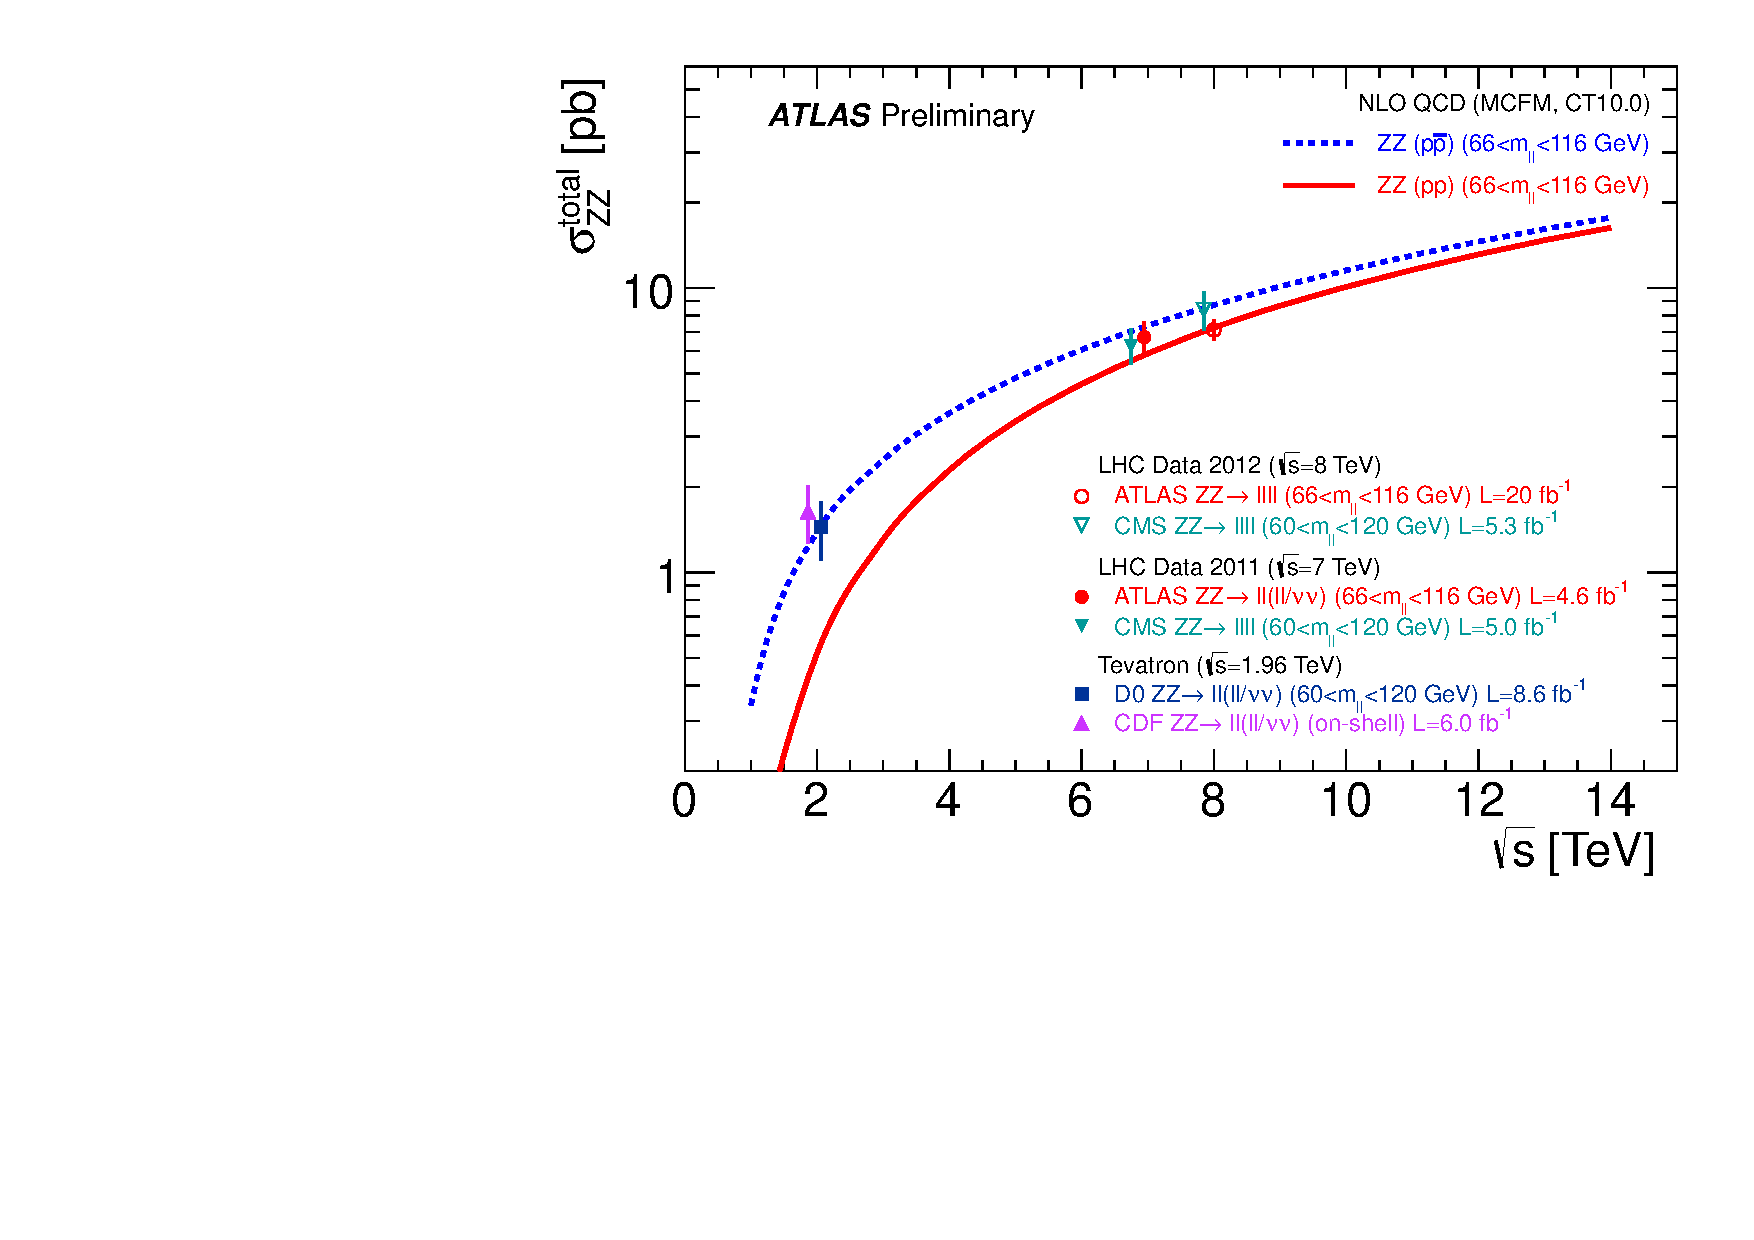
\includegraphics[width=0.9\textwidth]{SigmaZZatNLO}}
\caption[Comparison of experimental measurements and theoretical predictions of the total
\ZZ\ production \cx\ as a function of centre-of-mass energy $\sqrt{s}$.]{
\small
Comparison of experimental measurements and theoretical predictions of the total
\ZZ\ production \cx\ as a function of centre-of-mass energy $\sqrt{s}$. Shown
are experimental measurements from CDF~\cite{CDF:2011ab} and
D0~\cite{Abazov:2012cj} in $p\bar{p}$ collisions at the Tevatron at $\sqrt{s} =
1.96$~TeV, and experimental measurements from ATLAS and
CMS~\cite{CMS:2012rg,CMS:2013oev} in $pp$ collisions at the LHC at $\sqrt{s} =
7$~TeV and $\sqrt{s} = 8$~TeV. The blue dashed line shows the theoretical
prediction for the \ZZ\ production \cx\ in $p\bar{p}$ collisions,
calculated at NLO in QCD using MCFM with PDF set CT10. The solid red line shows
the theoretical prediction for the \ZZ\ production \cx\ in $pp$
collisions, calculated in the same way.  The theoretical curves are calculated
using the natural width of the $Z$ boson in the mass range 66 to 116 GeV.
 %At $\sqrt{s}=8$ TeV, the theoretical prediction using the zero-width
 %approximation is 5\% higher than the prediction using the natural width,
 %restricted to the mass range 66 to 116 GeV.
 }
\label{fig:sqrts-plot}
\end{center}
\end{figure}



\section{Unfolded Kinematic Distributions}
\label{sec:results-unfolded}

The observed kinematic distributions shown in~\sec{results-kindists} are a
convolution of the underlying `true' distribution of the parameter of interest
and distortion and smearing due to detector effects. Although 
%for the expected \ZZ\ signal distribution shown in these figures 
the detector distortion is included in the \mc\ simulation shown in those
figures, allowing a comparison of the theoretical prediction and the observed
data, it is desirable to correct the observed distributions for detector effects
in order to allow model-independent comparisons between theory and observation
and to allow comparison between different experiments. The correction procedure
is referred to as \intro{unfolding}. 

Formally, one can consider some parameter of interest $x$,
distributed according to a probability distribution function (\probDF) $f(x)$. Due to experimental effects, one
does not measure $x$ but a different (but related) variable $y$, distributed
according to a different \probDF\ $g(y)$. The measured variable $y$ is related to $x$ by a
convolution of the true distribution $f(x)$ with a response function $A(y,x)$ to account for the
experimental effects:
\begin{equation}
g(y) = \int A(y,x)f(x){\rm d}x 
\label{eqn:unfold-conv}
\end{equation}

In practice, continuous distributions are generally not measured, but instead
measurements are made
in discretised bins. $x$ and $y$ can thus be rewritten as
vectors \unfx\ and \unfy, where each element represents the number of events in
a given bin. The response
function then becomes a response matrix \unfA, and~\eqn{unfold-conv} can be
rewritten as:
\begin{equation}
\mathbf{y} = \mathbf{Ax} 
\label{eqn:unfold-conv-matrix}
\end{equation}

An iterative Bayesian algorithm~\cite{2010arXiv1010.0632D} is used to perform
the unfolding, 
using the implementation provided by the {\sc
RooUnfold}~\cite{2011arXiv1105.1160A} package. The algorithm treats the response
matrix \unfA\ as a description of the probability of observing some particular data given the
true distribution. From Bayes's theorem, the probability of there being in truth 
\unfxi\ events in bin $i$ of the true distribution arising due to
an observation of \unfyj\ events in bin $j$ is given by:
\begin{equation}
P(\unfxi|\unfyj,I) = \frac{P(\unfyj|\unfxi,I)\cdot P(\unfxi|I)}{\sum_{k}P(\unfyk|\unfxk,I)\cdot P(\unfxk|I)}
\end{equation}
where $I$ represents the state of information under which the analysis is
performed, and $P(\unfxi|I)$ is the prior for \unfxi. $P(\unfyi|\unfxj,I)$ is
given by element $A_{ij}$ of the unfolding matrix \unfA. $P(\unfxi|\unfyj,I)$
can be used to `share' the events observed in a single bin of \unfy\ between the bins of the
true distribution. An estimate of the true spectrum is obtained by 
`sharing' all of the bins of the observed distribution following this formula, taking into
account the efficiency. The estimate for \unfxi\ is thus given by:
\begin{equation}
\unfxi = \frac{1}{\epsilon_{i}} \, \sum^{n}_{j=1} \frac{A_{ji} \cdot
P(\unfxi|I)}{\sum_{k} A_{jk} \cdot P(\unfxk|I)} \cdot \unfyj
\end{equation}
where $\epsilon_{i}=\sum^{n}_{j} A_{j}$ accounts for the efficiency.

The initial set of priors $P(\unfxi|I)$ is taken from the simulated distribution from
\mc, and the unfolding matrix \unfA\ is also estimated using \mcsim. The
unfolding
procedure is iterated, taking the posterior distribution for \unfx\ from one iteration as a
prior for the next. The choice of initial prior will tend to bias the unfolded
distribution, but this bias decreases steeply with the number of iterations.
Conversely, the
statistical uncertainty tends to increase with the number of iterations, as
fluctuations can be amplified by positive feedback inherent in the algorithm;
the number of iterations must thus be chosen to balance the bias due to the
choice of prior and amplification of statistical uncertainties. It is found that
the difference in the results between three and four iterations is much smaller than
the statistical uncertainty. The results for three iterations are thus taken as
the nominal result, and the difference between three and four iterations is
taken as a systematic uncertainty. 

Statistical uncertainties due to the number of observed events are assessed by
pseudo-experiments, in each experiment fluctuating the observed \unfy\ by a
Poisson distribution and re-running the full unfolding procedure; the RMS of 2000
pseudo-experiments is taken as the statistical uncertainty. 
The response matrix \unfA\ has systematic uncertainties due to experimental
uncertainties; these are handled in a similar manner to the statistical
uncertainties, re-running the unfolding procedure multiple times and varying 
\unfA\ according to the different sources of uncertainty. An
additional systematic arises from the choice of prior. This is estimated by
using the distribution predicted by \sherpa\ as a prior instead of the nominal
\powhegbox. 

Distributions of three variables sensitive to new phenomena are selected for
unfolding: the transverse momentum \ptZ\ of the leading \Z\ boson candidate, the
angle \deltaPhiLL\ between the decay leptons of the leading \Z\ boson candidate,
and the four-lepton invariant mass \mZZ. Bin boundaries are chosen to maximise
sensitivity to nTGCs, and are in all cases larger than the detector resolution.
The unfolded distributions are presented in terms of a differential fiducial
\cx. This removes the effect of systematics that only affect the normalisation
and not the shape of the distribution. Unfolded distributions are only provided
for the 7~\tev\ analysis; they are shown in~\fig{unfolded-distributions}.  The
\sm\ prediction is consistent with the measurement in each case. The
uncertainty on the unfolded distributions is dominated by the statistical
uncertainty, which is approximately 30\% in most bins. The systematic
uncertainty is no more than 5\% in each bin, and is dominated by the
uncertainty arising due to the choice of prior.

\begin{figure}[htbp]
\begin{center}
\subfigure[]{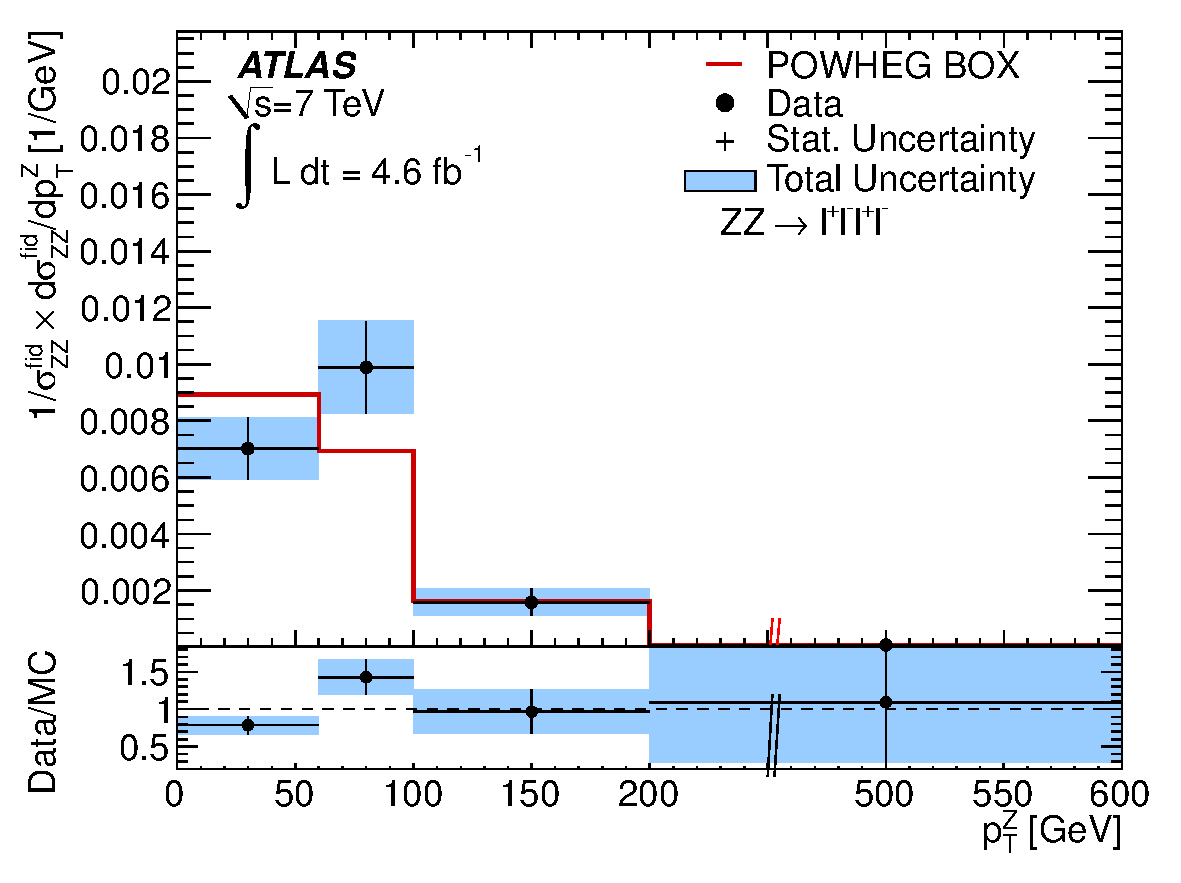
\includegraphics[width=0.57\textwidth]{Unfolded/ZZllll_ZpT_natbins_UnfoldedDistribution}}
\subfigure[]{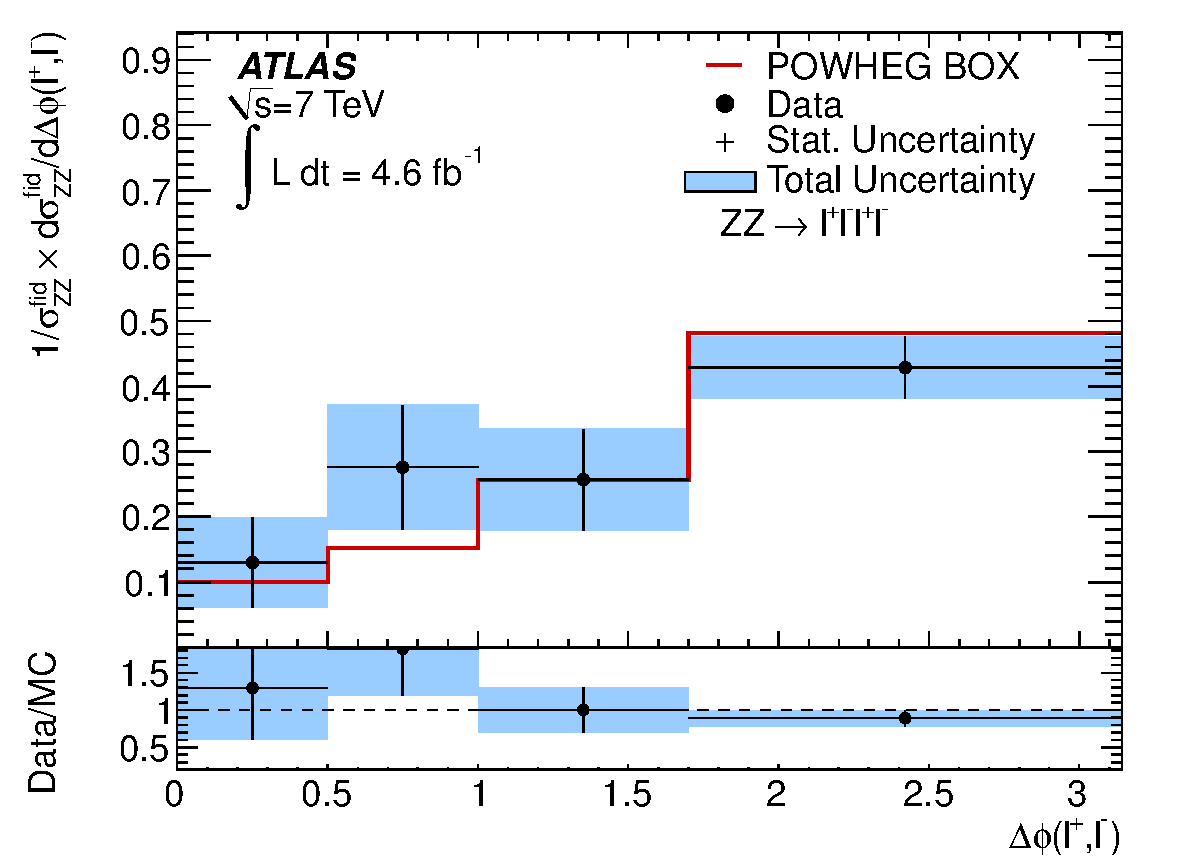
\includegraphics[width=0.57\textwidth]{Unfolded/ZZllll_DPhiLep_natbins_UnfoldedDistribution}}
\subfigure[]{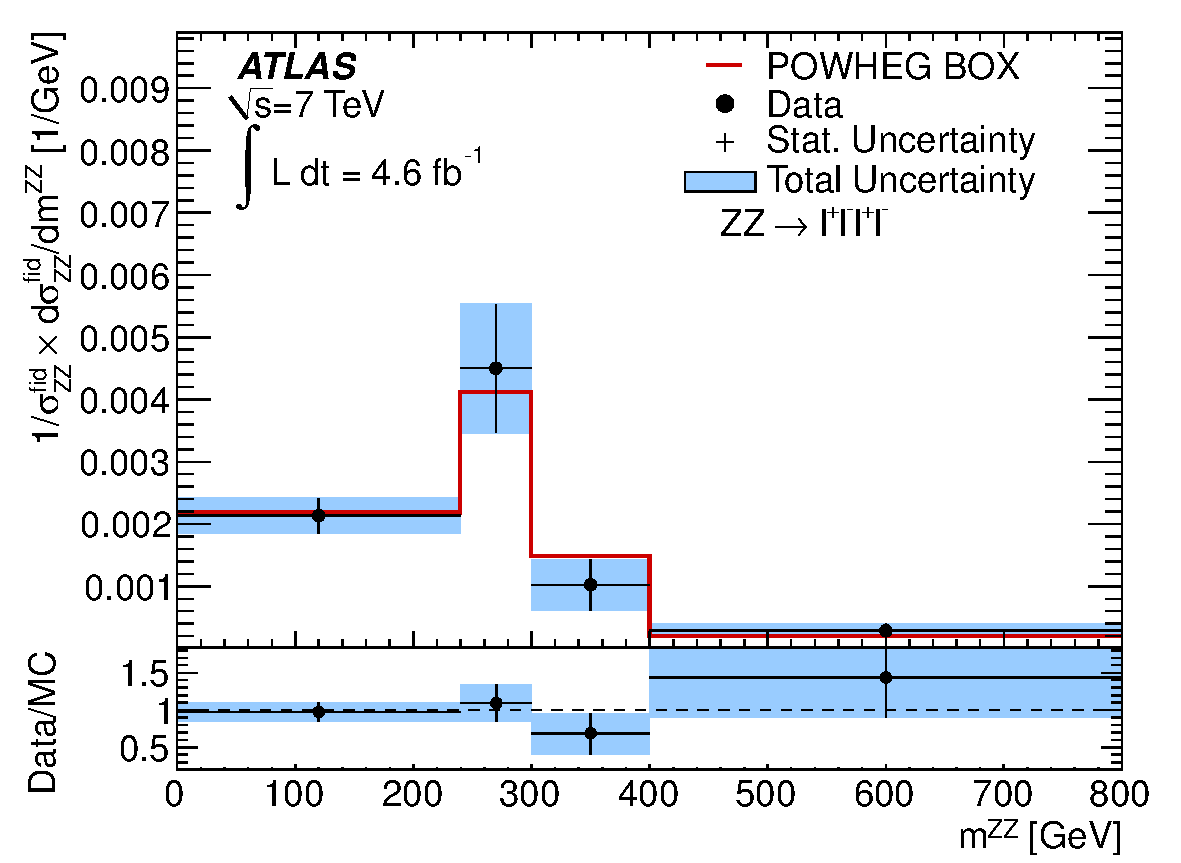
\includegraphics[width=0.57\textwidth]{Unfolded/ZZllll_ZZTMass_natbins_UnfoldedDistribution}}
\caption[Unfolded \ZZ\ fiducial \cx s.]{Unfolded \ZZ\ fiducial \cx s
in bins of (a) the
\pT\ of the leading \Z\ boson, (b) the angle between the decay leptons
of the leading \Z\ boson, \deltaPhiLL\ and (c) the four-lepton invariant mass,
\mZZ. The parallel lines in (a) indicate a binning discontinuity in the final bin.}
\label{fig:unfolded-distributions}
\end{center}
\end{figure}

